\nonstopmode
% Template KLTN cho SV trường ĐHKHTN
% Liên hệ: bhthong@fit.hcmus.edu.vn
% Last update: 

% Chú ý: đọc các phần chú ý đóng khung của file này và chỉnh lại cho phù hợp.
% Trước khi build, xóa hết các file được tạo ra trong quá trình build trước đó, và build theo thứ tự: BIB > PDF > PDF.
% Nếu cập nhật tài liệu tham khảo, cũng cần build lại theo cách trên.

\documentclass[oneside,a4paper,14pt]{extreport}

% Font tiếng Việt
\usepackage[T5]{fontenc}
\usepackage[utf8]{inputenc}
\usepackage{float}
\usepackage[section]{placeins}
\usepackage{longtable}
\DeclareTextSymbolDefault{\DH}{T1}

% Tài liệu tham khảo
%\usepackage[
%	sorting=nty,
%	backend=biber,
%    style=ieee
%	defernumbers=true]{biblatex}
\usepackage[style=ieee]{biblatex}
\usepackage[unicode]{hyperref} % Bookmark tiếng Việt
\addbibresource{References/references.bib}
%\bibliographystyle{IEEEtran}
%\bibliography{IEEEabrv,references}



\makeatletter
\def\blx@maxline{77}
\makeatother

% Chèn hình, các hình trong luận văn được để trong thư mục Images/
\usepackage{graphicx}
\graphicspath{ {Images/} }
\usepackage{pdfpages}

% Chèn và định dạng mã nguồn
\usepackage{listings}
\usepackage{color}
\definecolor{codegreen}{rgb}{0,0.6,0}
\definecolor{codegray}{rgb}{0.5,0.5,0.5}
\definecolor{codepurple}{rgb}{0.58,0,0.82}
\definecolor{backcolour}{rgb}{0.95,0.95,0.92}
\lstdefinestyle{mystyle}{
    backgroundcolor=\color{backcolour},   
    commentstyle=\color{codegreen},
    keywordstyle=\color{magenta},
    numberstyle=\tiny\color{codegray},
    stringstyle=\color{codepurple},
    basicstyle=\footnotesize,
    breakatwhitespace=false,         
    breaklines=true,                 
    captionpos=b,                    
    keepspaces=true,                 
    numbers=left,                    
    numbersep=5pt,                  
    showspaces=false,                
    showstringspaces=false,
    showtabs=false,                  
    tabsize=2
}
\lstset{style=mystyle}

% Chèn và định dạng mã giả
\usepackage{amsmath}
\usepackage{algorithm}
\usepackage[noend]{algpseudocode}
\makeatletter
\def\BState{\State\hskip-\ALG@thistlm}
\makeatother

% Bảng biểu
\usepackage{multirow}
\usepackage{array}
\usepackage{longtable}
\usepackage{rotating}
\newcolumntype{L}[1]{>{\raggedright\let\newline\\\arraybackslash\hspace{0pt}}m{#1}}
\newcolumntype{C}[1]{>{\centering\let\newline\\\arraybackslash\hspace{0pt}}m{#1}}
\newcolumntype{R}[1]{>{\raggedleft\let\newline\\\arraybackslash\hspace{0pt}}m{#1}}

% Đổi tên mặc định
\renewcommand{\chaptername}{Chương}
\renewcommand{\figurename}{Hình}
\renewcommand{\tablename}{Bảng}
\renewcommand{\contentsname}{Mục lục}
\renewcommand{\listfigurename}{Danh sách hình}
\renewcommand{\listtablename}{Danh sách bảng}
\renewcommand{\appendixname}{Phụ lục}


% Kích thước Chapter
\usepackage{titlesec}
\titleformat{\chapter}[display]
  {\LARGE\bfseries}
  {\chaptertitlename\ \thechapter}{18pt}{\huge}

% Đánh số và đưa vào mục lục tới cấp subsubsection (mục con chức năng ở Chương 5)
\setcounter{secnumdepth}{3}
\setcounter{tocdepth}{3}

% Nới tham số đặt hình (float) để hình và chữ chia sẻ trang tốt hơn,
% giảm khoảng trắng ở các trang nhiều ảnh (Chương 5 dùng [htbp]).
\renewcommand{\topfraction}{0.9}
\renewcommand{\bottomfraction}{0.85}
\renewcommand{\textfraction}{0.07}
\renewcommand{\floatpagefraction}{0.7}
\setcounter{topnumber}{3}
\setcounter{bottomnumber}{2}
\setcounter{totalnumber}{5}

% Giảm khoảng trắng dọc quanh hình/bảng và caption để bớt số trang
\setlength{\textfloatsep}{10pt plus 2pt minus 2pt}
\setlength{\floatsep}{8pt plus 2pt minus 2pt}
\setlength{\intextsep}{10pt plus 2pt minus 2pt}
\setlength{\abovecaptionskip}{5pt}
\setlength{\belowcaptionskip}{2pt}


% Dãn dòng 1.5
\usepackage{setspace}
\onehalfspacing

% Thụt vào đầu dòng
\usepackage{indentfirst}

% Canh lề
\usepackage[
  top=30mm,
  bottom=25mm,
  left=30mm,
  right=20mm,
  includefoot]{geometry}
  
% Trang bìa
\usepackage{tikz}
\usetikzlibrary{calc}
\newcommand\HRule{\rule{\textwidth}{1pt}}

% ========================================================================================= %
% CHÚ Ý: Thông tin chung về KLTN - sinh viên điền vào đây để tự động update các trang khác  %
% ========================================================================================= %
\newcommand{\tenSV}{Vòng~Sau~Hùng-Phan~Tấn~Phát-Nguyễn~Quốc~Tường-Huỳnh~Trần~Ty-Nguyễn~Trường~Vũ-Bùi~Đoàn~Thuý~Vy} % Dấu ~ là khoảng trắng không được tách (các chữ nối với nhau bằng dấu ~ sẽ nằm cùng 1 dòng
\newcommand{\mssv}{22120118-22120264-22120413-22120418-22120441-22120448}
\newcommand{\tenKL}{Xây~dựng~hệ~thống~hỗ~trợ~tìm~nhà~trọ~tích~hợp~AI} % Chú ý dấu ~ trong tên khóa luận
\newcommand{\tenGVHD}{ThS.~Phạm~Minh~Tuấn}
\newcommand{\tenBM}{Công nghệ phần mềm}

\begin{document}

\begin{titlepage}

\begin{center}
%ĐẠI HỌC QUỐC GIA THÀNH PHỐ HỒ CHÍ MINH\\
TRƯỜNG ĐẠI HỌC KHOA HỌC TỰ NHIÊN\\
\textbf{KHOA CÔNG NGHỆ THÔNG TIN}\\[2cm]


{ \bfseries Nhóm sinh viên:\\
Vòng Sau Hùng (22120118) \\
Phan Tấn Phát (22120264) \\
Nguyễn Quốc Tường (22120413) \\
Huỳnh Trần Ty (22120418) \\
Nguyễn Trường Vũ (22120441) \\
Bùi Đoàn Thuý Vy (22120448) \\[2cm]}

%Tên đề tài Khóa luận tốt nghiệp/Đồ án tốt nghiệp

{ \normalsize \bfseries XÂY DỰNG HỆ THỐNG HỖ TRỢ TÌM NHÀ TRỌ TÍCH HỢP AI \\[3cm]}


%Chọn trong các dòng sau
%\normalsize LUẬN VĂN THẠC SĨ KHOA HỌC MÁY TÍNH\\
\normalsize THỰC TẬP DỰ ÁN TỐT NGHIỆP\\
%Đưa vào dòng này nếu thuộc chương trình Chất lượng cao, hoặc lớp Cử nhân tài năng
\normalsize CHƯƠNG TRÌNH CHÍNH QUY\\[2cm]


\begin{tikzpicture}[remember picture, overlay]
  \draw[line width = 2pt] ($(current page.north west) + (2cm,-2cm)$) rectangle ($(current page.south east) + (-1.5cm,2cm)$);
\end{tikzpicture}

\vfill
Tp. Hồ Chí Minh, tháng 07/2026

\end{center}

\pagebreak



\begin{center}

TRƯỜNG ĐẠI HỌC KHOA HỌC TỰ NHIÊN\\
\textbf{KHOA CÔNG NGHỆ THÔNG TIN}\\[2cm]


{\bfseries Nhóm sinh viên thực hiện:\\
Vòng Sau Hùng (22120118)\\
Phan Tấn Phát (22120264)\\
Nguyễn Quốc Tường (22120413)\\
Huỳnh Trần Ty (22120418)\\
Nguyễn Trường Vũ (22120441)\\
Bùi Đoàn Thuý Vy (22120448)\\[1.5cm] }


%Tên đề tài Khóa luận tốt nghiệp/Đồ án tốt nghiệp

{ \normalsize \bfseries XÂY DỰNG HỆ THỐNG HỖ TRỢ TÌM NHÀ TRỌ TÍCH HỢP AI \\[2cm]}


%Chọn trong các dòng sau
%\normalsize LUẬN VĂN THẠC SĨ KHOA HỌC MÁY TÍNH\\
\normalsize THỰC TẬP DỰ ÁN TỐT NGHIỆP\\
%Đưa vào dòng này nếu thuộc chương trình Chất lượng cao, hoặc lớp Cử nhân tài năng
\normalsize CHƯƠNG TRÌNH CHÍNH QUY\\[1.5cm]

\textbf{NGƯỜI HƯỚNG DẪN}\\
ThS. Phạm Minh Tuấn\\


\begin{tikzpicture}[remember picture, overlay]
  \draw[line width = 2pt] ($(current page.north west) + (2cm,-2cm)$) rectangle ($(current page.south east) + (-1.5cm,2cm)$);
\end{tikzpicture}

\vfill
Tp. Hồ Chí Minh, tháng 07/2026

\end{center}

\end{titlepage}

% Sasu trang Title, các bạn chèn nhận xét gủa GVHD và GVPB. Nhận xét sẽ được giáo vụ phát sau buổi bảo vệ để các bạn đóng quyển.

\cleardoublepage

\pagenumbering{roman} % Đánh số i, ii, iii, ...


\phantomsection
\addcontentsline{toc}{chapter}{Lời cam đoan}
\chapter*{Lời cam đoan}
\label{commitment}
Chúng tôi xin cam đoan đây là công trình nghiên cứu của chúng tôi dưới sự hướng dẫn của giảng viên hướng dẫn ThS. Phạm Minh Tuấn. Chúng tôi xin chịu trách nhiệm về tính chính xác của các thông tin và kết quả nghiên cứu trong báo cáo này. Nếu có bất kỳ sai sót nào, chúng tôi xin hoàn toàn chịu trách nhiệm trước khoa Công nghệ thông tin, trường Đại học Khoa học Tự nhiên và các cơ quan liên quan.


% Nhận xét của GV hướng dẫn / phản biện: các bản nhận xét (kèm PDF) sẽ do giáo vụ
% cung cấp sau buổi bảo vệ. Bỏ chú thích các dòng dưới khi đã có file PDF tương ứng.
% \addcontentsline{toc}{chapter}{Nhận xét của GV hướng dẫn}
% \chapter*{Nhận xét hướng dẫn}
\label{advisor}

Bản nhận xét của giảng viên hướng dẫn (có chữ ký) do giáo vụ cung cấp.

\includepdf[pages=-]{../after-defense/GVHD.pdf}


% \addcontentsline{toc}{chapter}{Nhận xét của GV phản biện}
% \chapter*{Nhận xét phản biện}
\label{reviewer}

Bản nhận xét của giảng viên phản biện (có chữ ký) do giáo vụ cung cấp.

% TODO: Bỏ chú thích dòng dưới khi đã có file PDF nhận xét từ giáo vụ.
% \includepdf[pages=-]{../after-defense/GVPB.pdf}


\addcontentsline{toc}{chapter}{Lời cảm ơn}
\chapter*{Lời cảm ơn}
\label{thanks}

Nhóm sinh viên chúng em xin được gửi lời cảm ơn chân thành và sâu
sắc đến:

Ban Giám hiệu Trường Đại học Khoa học Tự nhiên – Đại học Quốc gia
Thành phố Hồ Chí Minh, cùng Ban Chủ nhiệm Khoa Công nghệ Thông
tin đã tạo điều kiện thuận lợi, cung cấp môi trường học tập và nghiên cứu tích cực để chúng em có thể thực hiện và hoàn thành đồ án tốt nghiệp với chủ đề “Xây dựng hệ thống hỗ trợ tìm nhà trọ tích hợp AI”.

Chúng em xin bày tỏ lòng biết ơn sâu sắc đến ThS. Phạm Minh Tuấn – là giảng viên hướng dẫn, người đã tận tình đồng hành, theo sát tiến độ của nhóm trong suốt quá trình thực hiện đồ án. Thầy không chỉ dành thời gian góp ý chuyên môn một cách cụ thể, xác đáng, mà còn truyền cảm hứng và định hướng cho nhóm áp dụng những công nghệ hiện đại và phù hợp, giúp sản phẩm đạt được tính ứng dụng thực tiễn cao.

Trong quá trình thực hiện đề tài, mặc dù đã rất nỗ lực nhưng chắc chắn không thể tránh khỏi những thiếu sót nhất định. Chúng em rất mong nhận được sự góp ý quý báu từ quý thầy cô để có thể hoàn thiện sản phẩm và nâng cao năng lực chuyên môn hơn nữa.

Những kiến thức, kỹ năng và trải nghiệm mà chúng em thu nhận được trong suốt quá trình làm đồ án sẽ là hành trang quý báu cho sự phát triển nghề nghiệp trong tương lai.

Một lần nữa, nhóm xin trân trọng cảm ơn tất cả quý thầy cô và những cá nhân đã hỗ trợ, đồng hành cùng nhóm trong chặng đường thực hiện đồ án tốt nghiệp này.


\addcontentsline{toc}{chapter}{Đề cương}
\chapter*{Đề cương chi tiết}
\label{proposal}

% TODO: Chèn file PDF đề cương chi tiết khi có, ví dụ:
% \includepdf[pages=-]{../proposal/proposal.pdf}


% Mục lục, danh sách hình, danh sách bảng
\addcontentsline{toc}{chapter}{Mục lục}

\tableofcontents

%\listoffigures
\cleardoublepage
% \phantomsection
\addcontentsline{toc}{chapter}{\listfigurename}
\listoffigures

\cleardoublepage
% \phantomsection
\addcontentsline{toc}{chapter}{\listtablename}
\listoftables
%\listoftables

\addcontentsline{toc}{chapter}{Danh mục từ viết tắt và thuật ngữ}
\chapter*{Danh mục từ viết tắt và thuật ngữ}
\label{Appendix1}

\begin{longtable}{|L{0.18\textwidth}|L{0.27\textwidth}|L{0.49\textwidth}|}
\hline
\textbf{Từ viết tắt} & \textbf{Từ đầy đủ} & \textbf{Giải thích} \\
\hline
\endfirsthead

\hline
\textbf{Từ viết tắt} & \textbf{Từ đầy đủ} & \textbf{Giải thích} \\
\hline
\endhead

\hline
\endfoot

AI & Artificial Intelligence & Lĩnh vực khoa học máy tính nghiên cứu các hệ thống có khả năng thực hiện tác vụ đòi hỏi trí thông minh con người. \\
\hline

LLM & Large Language Model & Mô hình học sâu với hàng tỷ tham số, có khả năng hiểu và tạo sinh ngôn ngữ tự nhiên. \\
\hline

RAG & Retrieval-Augmented Generation & Kỹ thuật kết hợp tìm kiếm thông tin từ cơ sở dữ liệu với khả năng tạo sinh của LLM để cải thiện độ chính xác. \\
\hline

API & Application Programming Interface & Tập hợp quy tắc và giao thức cho phép các phần mềm giao tiếp với nhau. \\
\hline

REST & Representational State Transfer & Kiểu kiến trúc thiết kế API trên nền giao thức HTTP, dùng cho giao tiếp giữa giao diện web và máy chủ. \\
\hline

SSR & Server-Side Rendering & Kỹ thuật kết xuất trang web phía máy chủ trước khi gửi về trình duyệt, giúp tối ưu tốc độ hiển thị lần đầu và SEO. \\
\hline

SEO & Search Engine Optimization & Tối ưu hóa để website thân thiện và dễ được các công cụ tìm kiếm xếp hạng cao. \\
\hline

SSE & Server-Sent Events & Cơ chế cho phép máy chủ đẩy dữ liệu liên tục về trình duyệt theo một chiều; được dùng cho luồng trả lời thời gian thực của trợ lý AI. \\
\hline

JWT & JSON Web Token & Chuẩn mã thông báo được ký số dùng để xác thực và truyền thông tin phiên đăng nhập một cách an toàn. \\
\hline

OAuth & Open Authorization & Giao thức ủy quyền cho phép đăng nhập thông qua tài khoản của bên thứ ba (ví dụ Google) mà không chia sẻ mật khẩu. \\
\hline

UI & User Interface & Giao diện người dùng -- phần người dùng nhìn thấy và tương tác trực tiếp với hệ thống. \\
\hline

WebSocket & WebSocket & Giao thức truyền dữ liệu hai chiều theo thời gian thực giữa trình duyệt và máy chủ trên một kết nối bền; dùng cho thông báo tức thời. \\
\hline

STOMP & Simple Text Oriented Messaging Protocol & Giao thức nhắn tin dạng văn bản chạy bên trên WebSocket, dùng để đẩy thông báo thời gian thực tới ứng dụng web. \\
\hline

SockJS & SockJS & Thư viện cung cấp kết nối kiểu WebSocket kèm cơ chế dự phòng (hỏi vòng) khi trình duyệt hoặc mạng không hỗ trợ WebSocket. \\
\hline

ICU & International Components for Unicode & Bộ định dạng chuỗi đa ngôn ngữ (số nhiều, tham số, ngày giờ) giúp hiển thị đúng ngữ pháp khi dịch giữa các ngôn ngữ. \\
\hline

NLP & Natural Language Processing & Xử lý ngôn ngữ tự nhiên -- một lĩnh vực thuộc trí tuệ nhân tạo nghiên cứu sự tương tác giữa máy tính và ngôn ngữ tự nhiên của con người. \\
\hline

RBAC & Role-Based Access Control & Kiểm soát truy cập dựa trên vai trò -- phương thức phân quyền và quản lý quyền hạn người dùng dựa trên vai trò cụ thể trong hệ thống. \\
\hline

PWA & Progressive Web Application & Ứng dụng web tiến trình -- giải pháp xây dựng ứng dụng web mang lại trải nghiệm và hiệu năng mượt mà tương tự ứng dụng di động gốc. \\
\hline

SOA & Service-Oriented Architecture & Kiến trúc hướng dịch vụ -- kiểu thiết kế phần mềm trong đó các thành phần ứng dụng cung cấp dịch vụ cho các thành phần khác thông qua giao thức truyền thông. \\
\hline

HTTP/HTTPS & HyperText Transfer Protocol (Secure) & Giao thức truyền tải dữ liệu trên nền web; phiên bản HTTPS bổ sung lớp mã hóa để bảo mật đường truyền. \\
\hline

JSON & JavaScript Object Notation & Định dạng văn bản nhẹ để biểu diễn và trao đổi dữ liệu có cấu trúc giữa các thành phần của hệ thống. \\
\hline

CI/CD & Continuous Integration / Continuous Deployment & Quy trình tự động tích hợp, kiểm thử và triển khai mã nguồn liên tục mỗi khi có thay đổi. \\
\hline

DTO & Data Transfer Object & Đối tượng truyền tải dữ liệu giữa các tầng, tách biệt cấu trúc dữ liệu trao đổi khỏi mô hình nghiệp vụ bên trong. \\
\hline

Modular Monolith & Modular Monolith & Kiến trúc nguyên khối mô-đun: ứng dụng chạy như một khối duy nhất nhưng được chia tách rõ ràng thành các module nghiệp vụ độc lập, sẵn sàng tách thành dịch vụ nhỏ khi cần. \\
\hline

Clean Architecture & Clean Architecture & Kiến trúc sạch: tổ chức mã nguồn theo nhiều tầng nhằm tách biệt logic nghiệp vụ khỏi các framework và chi tiết hạ tầng bên ngoài. \\
\hline

ReAct & Reasoning and Acting & Mô hình vận hành tác tử AI trong đó mô hình ngôn ngữ luân phiên suy luận và gọi công cụ cho tới khi đủ dữ kiện để trả lời. \\
\hline

ICL & In-Context Learning & Phương pháp học ngữ cảnh: cung cấp các ví dụ hoặc dữ liệu tham chiếu ngay trong câu lệnh (prompt) để mô hình ngôn ngữ suy luận mà không cần huấn luyện lại. \\
\hline

MCP & Model Context Protocol & Giao thức chuẩn hóa việc cung cấp ngữ cảnh và công cụ cho mô hình ngôn ngữ, cho phép các trợ lý AI bên ngoài truy vấn dữ liệu hệ thống. \\
\hline

CBF & Content-Based Filtering & Lọc theo nội dung: thuật toán gợi ý dựa trên độ tương đồng đặc trưng giữa các tin đăng. \\
\hline

CF & Collaborative Filtering & Lọc cộng tác: thuật toán gợi ý dựa trên hành vi tương tác của những người dùng tương tự nhau. \\
\hline

OTP & One-Time Password & Mã xác thực dùng một lần, có hiệu lực trong thời gian ngắn, dùng để xác minh danh tính người dùng. \\
\hline

Scrum & Scrum & Khung quản lý dự án theo phương pháp Agile, tổ chức công việc thành các chu kỳ (sprint) ngắn kèm họp định kỳ để tổng kết và lập kế hoạch. \\
\hline

% TODO: Bổ sung thêm các từ viết tắt và thuật ngữ khác khi hoàn thiện nội dung báo cáo.

\end{longtable}


\addcontentsline{toc}{chapter}{Tóm tắt}
\chapter*{Tóm tắt}
\label{summary}

% TODO: Viết phần tóm tắt đồ án (trong file Báo Cáo Cuối Kỳ phần này còn để trống).



\clearpage

\pagenumbering{arabic} % Đánh số 1, 2, 3, ...

% Các chương nội dung
\chapter{Giới thiệu đề tài}
\label{Chapter1}

\section{Đặt vấn đề}

% TODO: Nội dung (phần này còn để trống trong file Báo Cáo Cuối Kỳ).

\section{Mục tiêu đề tài}

% TODO: Nội dung (phần này còn để trống trong file Báo Cáo Cuối Kỳ).

\section{Phạm vi của đề tài}

% TODO: Nội dung (phần này còn để trống trong file Báo Cáo Cuối Kỳ).


\chapter{Tổng quan}
\label{Chapter2}

\section{Tổng quan về hệ thống thuê nhà trọ trực tuyến}

Các hệ thống tìm kiếm và giao dịch bất động sản cho thuê trực tuyến giữ vai trò quan trọng trong việc kết nối cung và cầu, trong đó phân khúc nhà trọ và phòng cho thuê bình dân chiếm tỷ trọng lớn tại các nước đang phát triển, đặc biệt là Việt Nam. Phần này trình bày khái quát các khái niệm cơ bản liên quan đến thị trường cho thuê nhà trọ, cùng các mô hình hệ thống công nghệ đang vận hành phổ biến hiện nay.

\FloatBarrier
\subsection{Khái niệm nhà trọ và thị trường cho thuê nhà trọ}

Nhà trọ hay phòng trọ cho thuê là một loại hình bất động sản cư trú quy mô nhỏ, được xây dựng hoặc phân tách từ một ngôi nhà nguyên căn nhằm mục đích cho cá nhân hoặc hộ gia đình thuê lại để ở trong một thời hạn nhất định. Đối tượng thuê nhà trọ chủ yếu tập trung vào các nhóm dân cư có tính dịch chuyển cao và thu nhập trung bình thấp như: sinh viên các trường đại học, người lao động ngoại tỉnh nhập cư, công nhân tại các khu công nghiệp, và các hộ gia đình trẻ chưa có đủ tích lũy tài chính để sở hữu nhà riêng.

Thị trường cho thuê nhà trọ tại các đô thị lớn của Việt Nam (đặc biệt là Hà Nội và TP. Hồ Chí Minh) mang tính đặc thù cao:
\begin{itemize}
    \item \textbf{Cầu vượt cung và mất cân bằng thông tin:} Lượng người đổ về các thành phố lớn học tập và làm việc tăng trưởng liên tục qua các năm, trong khi quỹ đất và nguồn cung phòng trọ giá rẻ có giới hạn. Điều này tạo nên thị trường do người bán quyết định, dẫn tới tình trạng chủ nhà trọ nắm thế chủ động và người thuê dễ rơi vào thế bị động khi tìm phòng.
    \item \textbf{Sự phân tán dữ liệu:} Thông tin phòng trọ thường không được quản lý tập trung mà phân tán nhỏ lẻ qua các biển treo thủ công, các hội nhóm mạng xã hội (Facebook, Zalo) hoặc các trang rao vặt không chuyên.
    \item \textbf{Sự thiếu minh bạch về chi phí và chất lượng:} Giá thuê phòng, giá điện, giá nước và các phí dịch vụ kèm theo (vệ sinh, bảo vệ, internet) thường do chủ nhà tự quyết định và không có hệ thống đối chiếu rõ ràng. Chất lượng phòng trọ trên ảnh quảng cáo thường sai lệch rất nhiều so với thực tế bàn giao.
\end{itemize}

\FloatBarrier
\subsection{Các mô hình hệ thống thuê nhà hiện nay}

Hiện nay, các giải pháp tìm kiếm và giao dịch bất động sản cho thuê trực tuyến tại Việt Nam và trên thế giới đang vận hành theo ba mô hình công nghệ chính:
\begin{enumerate}
    \item \textbf{Mô hình bảng tin rao vặt truyền thống:} Các website vận hành như một bảng tin công cộng (ví dụ: Phongtro123, các group Facebook). Người cho thuê đăng tin tự do và người thuê tự liên hệ trực tiếp. Ưu điểm là lượng tin phong phú và chi phí đăng thấp. Nhược điểm lớn là không kiểm soát được chất lượng tin đăng, tỷ lệ tin ảo, tin trùng lặp hoặc lừa đảo cao, gây lãng phí lớn về thời gian cho người dùng.
    \item \textbf{Mô hình sàn giao dịch tích hợp dịch vụ:} Các nền tảng đứng ra làm trung gian kiểm soát thông tin bài đăng và hỗ trợ các tính năng giá trị gia tăng như bản đồ tìm kiếm, thanh toán hóa đơn trực tuyến, và phân quyền môi giới chuyên nghiệp (ví dụ: Nhà Tốt, Batdongsan.com.vn). Mô hình này cải thiện tính minh bạch nhưng phần lớn quy trình vận hành vẫn chạy bằng nhân lực thủ công (nhân viên duyệt tin, nhân viên tư vấn gọi điện), dẫn đến tốc độ xử lý chậm và khó mở rộng quy mô một cách tối ưu.
    \item \textbf{Mô hình nền tảng thông minh tích hợp trí tuệ nhân tạo:} Là mô hình thế hệ mới mà đề tài này hướng đến xây dựng (Thuê Nhà Trọ). Hệ thống tận dụng sức mạnh của các mô hình ngôn ngữ lớn và học máy để tự động hóa hoàn toàn các tác vụ phức tạp: AI Agent hỗ trợ tư vấn và so sánh phòng bằng ngôn ngữ tự nhiên, AI tự động kiểm duyệt hình ảnh và nội dung tin đăng để lọc tin rác, AI định giá dựa trên ngữ cảnh thị trường, và gợi ý tin cá nhân hóa theo hành vi thời gian thực. Mô hình này giúp cải thiện trải nghiệm người dùng, giảm đáng kể chi phí vận hành thủ công và nâng cao độ an toàn giao dịch.
\end{enumerate}

\section{Khảo sát các nền tảng hiện có}

Trước khi đề xuất giải pháp, nhóm tiến hành khảo sát một số nền tảng tiêu biểu trong lĩnh vực rao vặt và tìm kiếm bất động sản cho thuê, bao gồm ba nền tảng phổ biến tại Việt Nam (Batdongsan.com.vn, Phongtro123, Nhà Tốt) và một nền tảng quốc tế đại diện cho hướng ứng dụng dữ liệu và công nghệ ở mức cao (Zillow). Việc khảo sát nhằm nhận diện các tính năng đã được thị trường chấp nhận, đồng thời chỉ ra những hạn chế còn tồn tại để làm cơ sở cho định hướng của đề tài.

\FloatBarrier
\subsection{Batdongsan.com.vn}

Batdongsan.com.vn~\cite{Batdongsan} là một trong những nền tảng rao vặt bất động sản lớn và lâu đời nhất tại Việt Nam, cung cấp tin đăng cho cả nhu cầu mua bán lẫn cho thuê trên phạm vi toàn quốc. Điểm mạnh của nền tảng là kho tin đăng lớn, công cụ tìm kiếm và lọc theo nhiều tiêu chí (khu vực, khoảng giá, diện tích, loại hình), cùng mô hình kinh doanh dựa trên các gói tin VIP và đẩy tin giúp người đăng tăng khả năng tiếp cận. Tuy nhiên, nền tảng thiên về phục vụ môi giới chuyên nghiệp và phân khúc mua bán; trải nghiệm cho người thuê ở phân khúc nhà trọ, phòng trọ giá rẻ chưa phải là trọng tâm, và chất lượng tin đăng phụ thuộc nhiều vào người đăng.

\FloatBarrier
\subsection{Phongtro123}

Phongtro123~\cite{Phongtro123} là nền tảng tập trung chuyên biệt vào phân khúc \textit{phòng trọ, nhà trọ} và các loại hình cho thuê giá rẻ, hướng tới đối tượng sinh viên và người lao động. Giao diện đơn giản, dễ sử dụng, cho phép lọc nhanh theo khu vực và mức giá, phù hợp với nhu cầu tìm trọ phổ thông. Bù lại, nền tảng chủ yếu dừng ở vai trò bảng tin rao vặt: thông tin tin đăng còn sơ sài, thiếu các công cụ hỗ trợ ra quyết định như so sánh, định giá tham khảo, bản đồ trực quan hay gợi ý cá nhân hóa, và việc kiểm soát chất lượng/độ tin cậy của tin đăng còn hạn chế.

\FloatBarrier
\subsection{Nhà Tốt}

Nhà Tốt~\cite{NhaTot} (chuyên mục bất động sản của nền tảng rao vặt Chợ Tốt) cung cấp tin đăng cho thuê và mua bán theo mô hình rao vặt giữa người dùng với người dùng. Nhờ thừa hưởng lượng người dùng lớn của Chợ Tốt, nền tảng có lưu lượng truy cập cao và đa dạng loại hình. Nền tảng có hỗ trợ bản đồ và một số tiện ích tìm kiếm, song giống các nền tảng nội địa khác, mức độ ứng dụng trí tuệ nhân tạo để định giá, gợi ý hay hỗ trợ hội thoại vẫn còn mờ nhạt, và trải nghiệm còn nặng tính rao vặt thủ công.

\FloatBarrier
\subsection{Zillow}

Zillow~\cite{Zillow} là nền tảng bất động sản hàng đầu tại Hoa Kỳ, nổi bật với việc ứng dụng dữ liệu và công nghệ ở mức cao. Tính năng tiêu biểu là \textit{Zestimate}, mô hình ước tính giá trị bất động sản tự động dựa trên dữ liệu thị trường, cùng với bản đồ giàu thông tin, dữ liệu khu vực chi tiết và trải nghiệm người dùng được trau chuốt. Zillow cho thấy tiềm năng to lớn của việc tích hợp dữ liệu và AI vào lĩnh vực bất động sản. Tuy vậy, nền tảng được thiết kế cho thị trường Hoa Kỳ với đặc thù dữ liệu, pháp lý và hành vi người dùng khác biệt, do đó không trực tiếp phù hợp với thị trường thuê trọ tại Việt Nam.

\FloatBarrier
\subsection{So sánh ưu nhược điểm}

Bảng~\ref{tab:compare-platforms} tổng hợp một số tiêu chí so sánh giữa các nền tảng đã khảo sát.

\begin{table}[!ht]
\centering
\small
\caption{So sánh tính năng giữa đề tài và các nền tảng hiện có}
\label{tab:compare-platforms}
\begin{tabular}{|L{0.22\textwidth}|C{0.11\textwidth}|C{0.11\textwidth}|C{0.10\textwidth}|C{0.10\textwidth}|C{0.13\textwidth}|}
\hline
\textbf{Tiêu chí} & \textbf{Batdong\-san} & \textbf{Phong\-tro123} & \textbf{Nhà Tốt} & \textbf{Zillow} & \textbf{Thuê Nhà Trọ} \\
\hline
Tập trung nhà trọ giá rẻ & Trung bình & Cao & Trung bình & Thấp & Cao \\
\hline
Tìm kiếm \& lọc đa tiêu chí & Cao & Trung bình & Trung bình & Cao & Cao \\
\hline
Bản đồ trực quan & Có & Hạn chế & Có & Cao & Có \\
\hline
Định giá thông minh & Không & Không & Không & Có & Có \\
\hline
Gợi ý cá nhân hóa & Hạn chế & Không & Hạn chế & Có & Có \\
\hline
Trợ lý hội thoại thông minh & Không & Không & Không & Hạn chế & Có \\
\hline
Phù hợp thị trường Việt Nam & Cao & Cao & Cao & Thấp & Cao \\
\hline
\end{tabular}
\end{table}

Qua so sánh có thể thấy: các nền tảng nội địa (Batdongsan.com.vn, Phongtro123, Nhà Tốt) phù hợp với thị trường và thói quen người dùng Việt Nam nhưng hầu như chưa khai thác trí tuệ nhân tạo để nâng cao trải nghiệm tìm kiếm và ra quyết định; trong khi đó, nền tảng quốc tế Zillow thể hiện rõ giá trị của việc tích hợp dữ liệu và AI nhưng lại không được thiết kế cho bối cảnh Việt Nam. Thuê Nhà Trọ lấp đầy khoảng trống đó: đặt trọng tâm vào phân khúc nhà trọ giá rẻ tại Việt Nam, đồng thời tích hợp đầy đủ các năng lực AI (định giá tham khảo, gợi ý cá nhân hóa và trợ lý hội thoại) mà các nền tảng hiện có chưa đáp ứng được.

\section{Cơ sở lý thuyết về trí tuệ nhân tạo}

Để khắc phục các hạn chế của phương pháp truyền thống, đề tài nghiên cứu và ứng dụng một số công nghệ trí tuệ nhân tạo, bao gồm các mô hình ngôn ngữ lớn, kỹ thuật tạo sinh kết hợp truy xuất, tác nhân AI và các mô hình gợi ý cá nhân hóa.

\FloatBarrier
\subsection{Mô hình ngôn ngữ lớn và Kỹ thuật Prompting}

Mô hình ngôn ngữ lớn là các mạng nơ-ron sâu dựa trên kiến trúc Transformer~\cite{Vaswani2017}, được huấn luyện trên các tập dữ liệu văn bản khổng lồ để hiểu và tạo sinh ngôn ngữ tự nhiên. Trong đề tài này, mô hình Gemini của Google được sử dụng làm nền tảng trí tuệ cốt lõi nhờ khả năng xử lý đa phương tiện và hiệu năng suy luận tốt \cite{GeminiDocs}.

Trong quá trình tích hợp LLM, kỹ thuật thiết kế chỉ thị đóng vai trò quyết định để định hình hành vi phản hồi của mô hình. Nhóm nghiên cứu đã ứng dụng hai kỹ thuật chính:
\begin{itemize}
    \item \textbf{In-Context Learning (Học ngữ cảnh / Few-Shot Prompting):} Thay vì tinh chỉnh lại trọng số mô hình vốn tốn kém tài nguyên, hệ thống cung cấp trực tiếp các ví dụ mẫu (inputs-outputs) hoặc các dữ liệu thực tế lân cận ngay trong prompt. Điều này giúp mô hình nhận diện cấu trúc, phong cách văn phong và quy luật định giá để phản hồi chính xác~\cite{Brown2020}.
    \item \textbf{System Prompting:} Thiết lập một tập quy tắc hành xử cố định cho mô hình.
\end{itemize}

\FloatBarrier
\subsection{Tạo sinh kết hợp truy xuất}

Mô hình ngôn ngữ lớn tuy rất thông minh nhưng lại mắc phải hai hạn chế nghiêm trọng: tri thức tĩnh (chỉ giới hạn trong thời điểm dữ liệu huấn luyện) và hiện tượng ``ảo tưởng'' (tự tạo ra thông tin sai lệch). Nhằm khắc phục hạn chế này, kỹ thuật tạo sinh kết hợp truy xuất đã được phát triển~\cite{Lewis2020}.

Quy trình RAG hoạt động theo ba bước chính:
\begin{enumerate}
    \item \textbf{Truy xuất (Retrieve):} Khi người dùng đặt câu hỏi (ví dụ: ``thủ tục đặt cọc nhà như thế nào?''), hệ thống sẽ chuyển hóa câu hỏi này và thực hiện tìm kiếm ngữ nghĩa trên cơ sở dữ liệu tri thức có sẵn (được lưu dưới dạng các tài liệu luật cư trú, cẩm nang thuê phòng trọ).
    \item \textbf{Tăng cường (Augment):} Đoạn văn bản kết quả tìm kiếm có độ liên quan cao nhất sẽ được đính kèm vào prompt gửi cho LLM như một tài liệu tham khảo chính thức.
    \item \textbf{Tạo sinh (Generate):} LLM đọc tài liệu này để tổng hợp câu trả lời chính xác, giúp hạn chế hiện tượng đoán mò và bảo đảm câu trả lời bám sát quy định pháp luật hoặc thông tin thực tế của hệ thống.
\end{enumerate}

\FloatBarrier
\subsection{Tác nhân trí tuệ nhân tạo và Vòng lặp ReAct}

Tác nhân AI là một thực thể phần mềm thông minh có khả năng tự động hóa quy trình ra quyết định để thực hiện một mục tiêu cụ thể bằng cách quan sát môi trường và kích hoạt các công cụ hành động (tools) có sẵn. Trong đề tài, trợ lý chatbot tìm phòng được xây dựng dưới dạng một Agent hoạt động theo vòng lặp ReAct (Reasoning and Acting)~\cite{Yao2023ReAct}.

Vòng lặp ReAct kết hợp đồng thời khả năng lập luận (Reasoning) và hành động (Acting) của LLM qua bốn giai đoạn lặp đi lặp lại:
\begin{itemize}
    \item \textbf{Suy nghĩ (Thought):} Agent phân tích câu lệnh của người dùng để xác định bước tiếp theo.
    \item \textbf{Hành động (Action):} Agent quyết định gọi một công cụ cụ thể với tham số đầu vào được trích xuất từ suy nghĩ.
    \item \textbf{Quan sát (Observation):} Hệ thống thực thi công cụ trong cơ sở dữ liệu và trả về kết quả thô cho Agent quan sát.
    \item \textbf{Lặp lại / Trả lời (Response):} Agent đánh giá kết quả quan sát. Nếu đã đủ thông tin, Agent sẽ sinh câu trả lời tự nhiên để phản hồi cho người dùng; nếu chưa đủ, Agent tiếp tục lập luận để thực hiện một hành động khác. Để tránh vòng lặp vô hạn do lỗi suy luận, hệ thống cấu hình giới hạn tối đa 12 bước thực thi cho mỗi câu hỏi.
\end{itemize}

\FloatBarrier
\subsection{Hệ thống gợi ý lai}

Hệ thống gợi ý tin đăng giúp cá nhân hóa trang chủ của từng người dùng dựa trên sở thích và hành vi của họ. Hệ thống Thuê Nhà Trọ triển khai cơ chế gợi ý lai~\cite{Burke2002} kết hợp hai hướng tiếp cận chính:
\begin{itemize}
    \item \textbf{Lọc dựa trên nội dung:} Gợi ý các tin đăng có đặc trưng tương đồng (tiện ích, khoảng giá, vị trí) với các tin đăng mà người dùng đó đã từng xem, lưu hoặc tương tác nhiều trong lịch sử. Độ tương đồng giữa các đặc trưng được tính toán bằng chỉ số độ tương đồng Cosine trên không gian vector.
    \item \textbf{Lọc cộng tác:} Tìm kiếm các người dùng có hành vi tương tự (lịch sử xem tin giống nhau) để gợi ý chéo các tin đăng mà người dùng tương tự kia đã thích nhưng người dùng hiện hành chưa biết tới.
\end{itemize}
Hai thuật toán này được tích hợp song song và chuẩn hóa điểm số, kết hợp với các hệ số hiệu chỉnh đặc thù (như khoảng cách địa lý từ cơ sở làm việc/học tập của người dùng và mức độ ưu tiên đẩy tin của tài khoản VIP) để xếp hạng danh sách gợi ý cuối cùng.

\section{Khoảng trống và cơ hội ứng dụng AI trong lĩnh vực cho thuê nhà trọ}

Qua khảo sát hiện trạng tại các nền tảng cho thuê bất động sản hiện nay (Batdongsan, Phongtro123, Nhà Tốt), nhóm nghiên cứu nhận diện rõ những khoảng trống công nghệ lớn và cơ hội ứng dụng trí tuệ nhân tạo để nâng tầm trải nghiệm của thị trường:

\begin{itemize}
    \item \textbf{Thay thế bộ lọc cứng nhắc bằng Giao diện hội thoại tự nhiên:} Các hệ thống hiện tại bắt buộc người thuê phải chọn hàng loạt bộ lọc phức tạp và thường dẫn tới kết quả rỗng khi điều kiện lọc quá khắt khe. Ứng dụng AI Agent cho phép người dùng mô tả nhu cầu dưới dạng một câu nói tự nhiên, Agent có khả năng tự động nới lỏng hoặc đề xuất phương án thay thế thông minh (ví dụ: gợi ý phòng ở quận lân cận khi quận đích đã hết phòng), mang lại trải nghiệm tìm kiếm mượt mà như đang giao tiếp trực tiếp với môi giới thật.
    \item \textbf{Giải quyết bài toán định giá thiếu minh bạch:} Người thuê và người cho thuê hiện nay định giá bất động sản chủ yếu dựa trên cảm tính hoặc tốn nhiều thời gian tự dò tìm so sánh thủ công. Tích hợp AI định giá kết hợp In-Context Learning giúp tự động phân tích hàng ngàn dữ liệu so sánh lân cận thời gian thực để đưa ra một báo cáo ước tính giá khách quan tức thời, hạn chế tối đa việc ép giá hoặc định giá quá cao.
    \item \textbf{Tự động hóa hoàn toàn quy trình kiểm duyệt chất lượng:} Quy trình kiểm duyệt tin thủ công bằng con người của các sàn truyền thống thường gây trễ bài đăng (từ vài giờ đến vài ngày) và dễ bỏ sót tin spam hoặc hình ảnh không phù hợp. Ứng dụng mô hình Gemini Multimodal cho phép quét lập tức hình ảnh, video và văn bản ngay khi chủ trọ vừa bấm đăng tin để phát hiện tin trùng, ảnh mờ, hoặc thông tin rác, giúp tăng tốc độ phê duyệt tin đăng lên thời gian thực trong khi vẫn đảm bảo độ tin cậy của dữ liệu trên sàn.
    \item \textbf{Cá nhân hóa tối đa trải nghiệm người dùng:} Phản lớn các trang rao vặt hiển thị tin đăng theo thứ tự thời gian hoặc mức phí dịch vụ thuần túy, dẫn tới việc người dùng bị ngợp bởi thông tin không liên quan. Việc triển khai hệ thống gợi ý lai (Collaborative + Content-based) giúp cá nhân hóa giao diện trang chủ theo đúng nhu cầu cư trú riêng biệt của từng cá nhân (khoảng cách đi lại tối ưu, sở thích tiện nghi), cải thiện tỷ lệ chuyển đổi giao dịch cho nền tảng.
\end{itemize}


\chapter{Phương pháp đề xuất}
\label{Chapter3}

\section{Kiến trúc tổng quan}

% TODO: Nội dung (phần này còn để trống trong file Báo Cáo Cuối Kỳ).

\subsection{Mô hình kiến trúc hệ thống}

% TODO: Nội dung.

\subsection{Khái quát các thành phần bên trong hệ thống}

% TODO: Nội dung.

\section{Nền tảng Web}

Nền tảng Web của hệ thống được tách thành hai ứng dụng độc lập nhưng dùng chung phong cách thiết kế và quy ước kỹ thuật: \textbf{ứng dụng web cho người dùng cuối} (webapp -- nơi người thuê tìm kiếm, so sánh, lưu tin và liên hệ chủ trọ; đồng thời là không gian để người môi giới/chủ nhà đăng và quản lý tin) và \textbf{trang quản trị} (admin -- dành cho quản trị viên). Phần này tập trung mô tả ứng dụng web cho người dùng cuối, vốn là thành phần người dùng tương tác trực tiếp nhiều nhất; phần trang quản trị được trình bày ở mục tiếp theo.

Webapp được xây dựng trên \textbf{Next.js 15} (theo mô hình Pages Router) cùng \textbf{React 19} và \textbf{TypeScript}, sử dụng Tailwind CSS v4 kết hợp bộ component shadcn/ui làm hệ thống giao diện. Việc lựa chọn Next.js cho phép kết xuất phía máy chủ (Server-Side Rendering -- SSR) đối với các trang quan trọng về SEO như trang chi tiết tin đăng và trang tin tức, đồng thời tận dụng được hệ sinh thái React phong phú cho phần tương tác phía trình duyệt \cite{ReactDocs,NextDocs}.

\subsection{Tổ chức mã nguồn}

Mã nguồn được tổ chức theo nguyên tắc \textit{tách bạch mối quan tâm} (separation of concerns) và \textit{thiết kế nguyên tử} (Atomic Design), với mục tiêu để mỗi tính năng có thể phát triển độc lập, dễ kiểm thử và dễ bảo trì. Toàn bộ mã nguồn nằm dưới thư mục \texttt{src/}, được phân chia thành các nhóm chính như Bảng~\ref{tab:webapp-structure}.

\begin{table}[H]
\centering
\caption{Cấu trúc thư mục mã nguồn của ứng dụng web}
\label{tab:webapp-structure}
\begin{tabular}{|L{0.30\textwidth}|L{0.60\textwidth}|}
\hline
\textbf{Thư mục} & \textbf{Vai trò} \\
\hline
\texttt{pages/} & Lớp định tuyến (Pages Router). Mỗi tệp là một ``vỏ mỏng'' chỉ lắp ghép dữ liệu vào template và gắn bố cục trang. \\
\hline
\texttt{components/} & Cây giao diện theo Atomic Design: \texttt{atoms} (nguyên tử shadcn), \texttt{molecules}, \texttt{organisms}, \texttt{templates} và \texttt{layouts}. \\
\hline
\texttt{api/services/} & Các module gọi API theo từng nghiệp vụ (tin đăng, môi giới, thanh toán, tin tức, thông báo, AI\ldots). \\
\hline
\texttt{hooks/} & Các React Hook tùy biến đóng gói logic nghiệp vụ và truy vấn dữ liệu. \\
\hline
\texttt{contexts/}, \texttt{store/} & Quản lý trạng thái dùng chung (xác thực, ngôn ngữ, danh sách so sánh\ldots) qua React Context và Zustand. \\
\hline
\texttt{configs/}, \texttt{constants/} & Cấu hình thư viện (axios, biến môi trường) và hằng số toàn cục. \\
\hline
\texttt{messages/}, \texttt{utils/}, \texttt{styles/} & Bộ từ điển đa ngôn ngữ, các hàm tiện ích thuần và mã định kiểu giao diện. \\
\hline
\end{tabular}
\end{table}

Cây giao diện tuân thủ nghiêm ngặt thứ tự phân lớp \texttt{atoms $\to$ molecules $\to$ organisms $\to$ templates $\to$ pages}, trong đó lớp dưới không bao giờ được phép nhập (import) từ lớp trên. Cụ thể, \textbf{atoms} là các nguyên tử giao diện cơ bản (nút bấm, ô nhập liệu, hộp thoại\ldots) được chuẩn hóa theo shadcn/ui; \textbf{molecules} ghép các nguyên tử thành các khối nhỏ như trường biểu mẫu, thẻ lọc; \textbf{organisms} là các khối tính năng hiểu biết về dữ liệu và quy tắc nghiệp vụ (thẻ tin đăng, hộp thoại đăng nhập, widget trợ lý AI\ldots); \textbf{templates} là bố cục đầy đủ của một họ trang; còn \textbf{pages} chỉ đóng vai trò lắp ráp. Mỗi thư mục thành phần đều cung cấp một tệp \texttt{index} làm điểm xuất khẩu tập trung (barrel export), giúp việc nhập khẩu nhất quán và che giấu cấu trúc nội bộ.

Song song với cây giao diện, logic được tách theo \textit{nghiệp vụ}: mỗi miền dữ liệu có một module dịch vụ (\texttt{*.service.ts}) chịu trách nhiệm gọi API và một nhóm hook (\texttt{use*}) bao bọc dịch vụ đó. Nhờ vậy, logic nghiệp vụ nằm ở hook và context, việc lấy dữ liệu nằm ở tầng dịch vụ, còn component chỉ lo phần hiển thị. Cách phân tách này giúp giảm thiểu sự phụ thuộc chéo và cho phép nhiều thành viên cùng phát triển các tính năng khác nhau mà ít xảy ra xung đột.

% TODO (Phát): chèn Hình -- Sơ đồ tổ chức mã nguồn webapp (ch32-source-org.png), minh họa các lớp atoms -> molecules -> organisms -> templates -> pages và quan hệ services/hooks.

\subsection{Cơ chế kết nối và tích hợp}

Ứng dụng web không tự chứa dữ liệu mà kết nối tới nhiều dịch vụ phía sau thông qua các kênh giao tiếp được chuẩn hóa:

\begin{itemize}
\item \textbf{Giao tiếp HTTP với Backend chính.} Mọi yêu cầu REST đi qua một thể hiện \texttt{axios} duy nhất được cấu hình tập trung tại \texttt{src/configs/axios}. Thể hiện này gắn sẵn URL gốc của Backend (biến môi trường \texttt{URL\_API\_BASE}), tiêu đề mặc định và bộ chặn (interceptor) xử lý xác thực. Toàn bộ phản hồi được chuẩn hóa về một kiểu \texttt{ApiResponse} thống nhất để các tầng phía trên xử lý nhất quán.

\item \textbf{Xác thực bằng JWT và cơ chế làm mới token.} Bộ chặn yêu cầu tự động đính kèm \textit{access token} vào tiêu đề \texttt{Authorization}. Khi token sắp hết hạn hoặc máy chủ trả về lỗi 401, hệ thống tự động gọi \textit{refresh token} để lấy token mới rồi phát lại yêu cầu ban đầu một cách trong suốt với người dùng. Cơ chế này còn khử trùng lặp (deduplication) để nhiều yêu cầu đồng thời chỉ kích hoạt đúng một lần làm mới, tránh tình trạng đua tranh (race condition).

\item \textbf{Cổng chặn truy cập (middleware).} Tệp \texttt{src/middleware.ts} đóng vai trò cổng kiểm soát: nó cho phép một danh sách các tuyến công khai (trang chủ, danh sách tin, chi tiết tin, tin tức, bản đồ\ldots) và chặn các tuyến cá nhân khi người dùng chưa đăng nhập. Khi đó, người dùng được chuyển hướng kèm tham số \texttt{returnUrl} để sau khi đăng nhập có thể quay lại đúng trang đang truy cập.

\item \textbf{Bộ nhớ đệm dữ liệu máy chủ.} Toàn bộ trạng thái lấy từ máy chủ được quản lý bởi \textbf{TanStack Query}, giúp tự động lưu đệm, làm mới nền và đồng bộ dữ liệu giữa các thành phần. Một số dữ liệu thống kê ổn định theo ngày (ví dụ thống kê tin theo tỉnh thành) còn được lưu bền vào \texttt{localStorage} để tồn tại qua các lần tải lại trang.

\item \textbf{Kết nối dịch vụ AI bằng luồng SSE.} Trợ lý hội thoại AI kết nối tới một dịch vụ AI riêng (biến môi trường \texttt{URL\_API\_AI}) và nhận câu trả lời theo thời gian thực qua kỹ thuật \textit{Server-Sent Events} (sử dụng thư viện \texttt{fetch-event-source}). Nhờ đó nội dung trả lời hiện dần theo từng đoạn, kèm theo trạng thái công cụ mà AI đang thực thi, và người dùng có thể hủy luồng đang chạy.

\item \textbf{Thông báo thời gian thực qua WebSocket.} Các thông báo (tin được duyệt, có người quan tâm\ldots) được đẩy theo thời gian thực qua giao thức \textbf{STOMP trên SockJS}, kết hợp với cơ chế hỏi vòng (polling) dự phòng khi mất kết nối.

\item \textbf{Tích hợp dịch vụ bên thứ ba.} Bản đồ tin đăng tích hợp Google Maps; luồng thanh toán điều hướng sang cổng thanh toán rồi nhận lại kết quả qua một trang callback công khai để cổng có thể chuyển hướng về.
\end{itemize}

\subsection{Hỗ trợ đa ngôn ngữ}

Ứng dụng hỗ trợ song ngữ \textbf{tiếng Việt} (mặc định) và \textbf{tiếng Anh}, được triển khai bằng thư viện \textbf{next-intl}. Mọi chuỗi hiển thị cho người dùng -- nhãn, nút bấm, thông báo, thông điệp lỗi, văn bản trạng thái rỗng -- đều không được viết cứng trong mã mà phải lấy qua các hàm \texttt{useTranslations} (phía client) hoặc \texttt{getTranslations} (phía server), tham chiếu tới hai bộ từ điển \texttt{messages/vi.json} và \texttt{messages/en.json}.

Một số điểm kỹ thuật đáng chú ý trong cơ chế đa ngôn ngữ:

\begin{itemize}
\item \textbf{Tải từ điển theo nhu cầu.} Vì phần lớn người dùng sử dụng tiếng Việt, bộ từ điển \texttt{vi.json} được đóng gói sẵn cùng ứng dụng; bộ \texttt{en.json} chỉ được tải động khi người dùng thực sự chuyển sang tiếng Anh, giúp giảm kích thước gói tải ban đầu.
\item \textbf{Bảo đảm đồng bộ khóa dịch.} Một kịch bản kiểm tra (\texttt{check-i18n-keys.js}) được chạy tự động trong bước \texttt{pre-commit} để đối chiếu sự tương đồng khóa giữa hai tệp ngôn ngữ; nếu thiếu khóa ở một ngôn ngữ, thao tác commit sẽ bị chặn.
\item \textbf{Dùng định dạng ICU.} Các chuỗi có tham số sử dụng placeholder kiểu ICU (\texttt{\{name\}}, \texttt{\{count, plural, \ldots\}}) thay vì nối chuỗi thủ công, bảo đảm đúng ngữ pháp khi trật tự từ khác nhau giữa các ngôn ngữ.
\item \textbf{Quản lý trạng thái ngôn ngữ.} Việc chuyển ngôn ngữ được điều phối qua một context riêng (\texttt{SwitchLanguageProvider}), ghi nhớ lựa chọn của người dùng và cung cấp bộ từ điển phù hợp cho toàn bộ cây thành phần.
\end{itemize}

% TODO (Phát): chèn Hình -- Ảnh chụp giao diện ở hai ngôn ngữ Việt/Anh (ch32-i18n.png).

\subsection{Ưu điểm}

Cách tổ chức và tích hợp nêu trên mang lại một số ưu điểm rõ rệt cho nền tảng web:

\begin{itemize}
\item \textbf{Dễ bảo trì và mở rộng.} Kiến trúc Atomic Design phân lớp rõ ràng cùng việc tách logic theo nghiệp vụ giúp định vị và sửa đổi mã nhanh chóng; thêm một tính năng mới thường chỉ cần bổ sung một template, một dịch vụ và một nhóm hook tương ứng mà không ảnh hưởng phần còn lại.
\item \textbf{An toàn kiểu dữ liệu.} Việc dùng TypeScript trên toàn dự án, giới hạn kiểu \texttt{any} chỉ trong tầng định nghĩa dữ liệu truyền tải, giúp phát hiện sớm lỗi ngay khi biên dịch.
\item \textbf{Hiệu năng và trải nghiệm tốt.} Kết hợp SSR cho các trang trọng yếu về SEO, tải động (lazy loading) các thành phần nặng như bản đồ và biểu đồ, cùng cơ chế lưu đệm của TanStack Query giúp trang hiển thị nhanh và mượt.
\item \textbf{Nhất quán về giao diện.} Hệ thống thiết kế tập trung (typography, khoảng cách, màu sắc theo token ngữ nghĩa) cùng các quy tắc lint riêng bảo đảm giao diện đồng nhất giữa các trang và giữa các thành viên phát triển.
\item \textbf{Thuận lợi cho cộng tác nhóm.} Quy ước thư mục, barrel export và các cổng kiểm soát chất lượng (lint, kiểm tra kiểu, kiểm tra khóa đa ngôn ngữ) tạo nền tảng để nhiều người cùng làm việc trên cùng mã nguồn mà vẫn giữ được chất lượng ổn định.
\end{itemize}

\section{Hệ thống Backend}

% TODO: Nội dung.

\subsection{Kiến trúc Modular Monolith}

% TODO: Nội dung.

\subsection{Các module nghiệp vụ}

% TODO: Nội dung.

\subsection{Tổ chức phân tầng bên trong module}

% TODO: Nội dung.

\subsection{Luồng dữ liệu}

% TODO: Nội dung.

\subsection{Ưu điểm}

% TODO: Nội dung.

\section{Hệ thống AI}

% TODO: Nội dung.

\subsection{AI Agent hỗ trợ tìm kiếm nhà trọ}

% TODO: Nội dung.

\subsection{Hệ thống đánh giá giá bất động sản}

% TODO: Nội dung.

\subsection{Hệ thống gợi ý cá nhân hóa}

% TODO: Nội dung.

\subsection{AI tạo nội dung bài đăng}

% TODO: Nội dung.

\subsection{Hệ thống gợi ý cá nhân hóa}

% TODO: Nội dung. (Lưu ý: mục này trùng tiêu đề với mục 3.4.3 trong file gốc -- cần rà soát lại.)

\subsection{AI kiểm tra nội dung bài đăng tại admin}

% TODO: Nội dung.

\subsection{Kiến trúc tích hợp AI}

% TODO: Nội dung.

\subsection{Ưu điểm}

% TODO: Nội dung.

\section{Hạ tầng}

% TODO: Nội dung.

\subsection{R2}

% TODO: Nội dung.

\subsection{MySQL}

% TODO: Nội dung.

\subsection{LiteLLM \& Langfuse}

% TODO: Nội dung.

\subsection{Cổng thanh toán}

% TODO: Nội dung.

\subsection{CI/CD Pipeline}

% TODO: Nội dung.

\subsection{Triển khai ứng dụng}

% TODO: Nội dung.

\section{Cơ sở dữ liệu}

% TODO: Nội dung.

\subsection{Giới thiệu tổng quan}

% TODO: Nội dung.

\subsection{Sơ đồ thiết kế cơ sở dữ liệu của hệ thống chính}

% TODO: Nội dung.

\subsection{Mô tả chi tiết các bảng}

% TODO: Nội dung.


\chapter{Thiết kế hệ thống}
\label{Chapter4}

\section{Kiến trúc tổng thể hệ thống}

% TODO: Nội dung (phần này còn để trống trong file Báo Cáo Cuối Kỳ).

\subsection{Mô hình kiến trúc hệ thống}

% TODO: Nội dung.

\subsection{Khái quát các thành phần bên trong hệ thống}

% TODO: Nội dung.

\section{Thiết kế nền tảng Web}

Nền tảng Web của hệ thống được tách thành hai ứng dụng độc lập: ứng dụng web cho người dùng cuối (webapp -- nơi người thuê tìm kiếm, so sánh, lưu tin và liên hệ chủ trọ; đồng thời là không gian để người môi giới/chủ nhà đăng và quản lý tin) và trang quản trị (admin -- dành cho quản trị viên). Mỗi ứng dụng có cơ sở mã, phong cách thiết kế và quy ước kỹ thuật riêng, phù hợp với nhóm người dùng mà nó phục vụ. Phần này tập trung mô tả ứng dụng web cho người dùng cuối, vốn là thành phần người dùng tương tác trực tiếp nhiều nhất; phần trang quản trị được trình bày ở mục tiếp theo.

Webapp được xây dựng trên Next.js 15 (theo mô hình Pages Router) cùng React 19 và TypeScript, sử dụng Tailwind CSS v4 kết hợp bộ component shadcn/ui làm hệ thống giao diện. Việc lựa chọn Next.js cho phép kết xuất phía máy chủ (Server-Side Rendering -- SSR) đối với các trang quan trọng về SEO như trang chi tiết tin đăng và trang tin tức, đồng thời tận dụng được hệ sinh thái React phong phú cho phần tương tác phía trình duyệt \cite{ReactDocs,NextDocs}.

\subsection{Tổ chức mã nguồn}

Mã nguồn được tổ chức theo nguyên tắc \textit{tách bạch mối quan tâm} (separation of concerns) và \textit{thiết kế nguyên tử} (Atomic Design), với mục tiêu để mỗi tính năng có thể phát triển độc lập, dễ kiểm thử và dễ bảo trì. Toàn bộ mã nguồn nằm dưới thư mục \texttt{src/}, được phân chia thành các nhóm chính như Bảng~\ref{tab:webapp-structure}.

\begin{table}[H]
\centering
\caption{Cấu trúc thư mục mã nguồn của ứng dụng web}
\label{tab:webapp-structure}
\begin{tabular}{|L{0.30\textwidth}|L{0.60\textwidth}|}
\hline
\textbf{Thư mục} & \textbf{Vai trò} \\
\hline
\texttt{pages/} & Lớp định tuyến (Pages Router). Mỗi tệp là một ``vỏ mỏng'' chỉ lắp ghép dữ liệu vào template và gắn bố cục trang. \\
\hline
\texttt{components/} & Cây giao diện theo Atomic Design: \texttt{atoms} (nguyên tử shadcn), \texttt{molecules}, \texttt{organisms}, \texttt{templates} và \texttt{layouts}. \\
\hline
\texttt{api/services/} & Các module gọi API theo từng nghiệp vụ (tin đăng, môi giới, thanh toán, tin tức, thông báo, AI\ldots). \\
\hline
\texttt{hooks/} & Các React Hook tùy biến đóng gói logic nghiệp vụ và truy vấn dữ liệu. \\
\hline
\texttt{contexts/}, \texttt{store/} & Quản lý trạng thái dùng chung (xác thực, ngôn ngữ, danh sách so sánh\ldots) qua React Context và Zustand. \\
\hline
\texttt{configs/}, \texttt{constants/} & Cấu hình thư viện (axios, biến môi trường) và hằng số toàn cục. \\
\hline
\texttt{messages/}, \texttt{utils/}, \texttt{styles/} & Bộ từ điển đa ngôn ngữ, các hàm tiện ích thuần và mã định kiểu giao diện. \\
\hline
\end{tabular}
\end{table}

Cây giao diện tuân thủ nghiêm ngặt thứ tự phân lớp \texttt{atoms $\to$ molecules $\to$ organisms $\to$ templates $\to$ pages}, trong đó lớp dưới không bao giờ được phép nhập (import) từ lớp trên. Cụ thể, \texttt{atoms} là các nguyên tử giao diện cơ bản (nút bấm, ô nhập liệu, hộp thoại\ldots) được chuẩn hóa theo shadcn/ui; \texttt{molecules} ghép các nguyên tử thành các khối nhỏ như trường biểu mẫu, thẻ lọc; \texttt{organisms} là các khối tính năng hiểu biết về dữ liệu và quy tắc nghiệp vụ (thẻ tin đăng, hộp thoại đăng nhập, widget trợ lý AI\ldots); \texttt{templates} là bố cục đầy đủ của một họ trang; còn \texttt{pages} chỉ đóng vai trò lắp ráp. Mỗi thư mục thành phần đều cung cấp một tệp \texttt{index} làm điểm xuất khẩu tập trung (barrel export), giúp việc nhập khẩu nhất quán và che giấu cấu trúc nội bộ.

Song song với cây giao diện, logic được tách theo \textit{nghiệp vụ}: mỗi miền dữ liệu có một module dịch vụ (\texttt{*.service.ts}) chịu trách nhiệm gọi API và một nhóm hook (\texttt{use*}) bao bọc dịch vụ đó. Nhờ vậy, logic nghiệp vụ nằm ở hook và context, việc lấy dữ liệu nằm ở tầng dịch vụ, còn component chỉ lo phần hiển thị. Cách phân tách này giúp giảm thiểu sự phụ thuộc chéo và cho phép nhiều thành viên cùng phát triển các tính năng khác nhau mà ít xảy ra xung đột.

Hình~\ref{fig:webapp-source-org} tổng hợp cách tổ chức mã nguồn webapp theo các lớp nêu trên. Lớp định tuyến (\texttt{pages}) nằm trên cùng; bên dưới là cây giao diện Atomic Design (\texttt{templates $\to$ organisms $\to$ molecules $\to$ atoms}) tách biệt với nhánh logic gồm \texttt{hooks}, \texttt{contexts}/\texttt{store} và tầng dịch vụ (\texttt{api/services}) chịu trách nhiệm gọi API qua \texttt{axios}. Mũi tên nét liền thể hiện quan hệ phụ thuộc khi kết xuất giao diện, còn mũi tên nét đứt thể hiện việc các thành phần sử dụng hook để lấy dữ liệu; nhờ đó component chỉ lo phần hiển thị, còn logic nghiệp vụ và truy xuất dữ liệu được đẩy xuống các tầng phía dưới.

\begin{figure}[H]
\centering
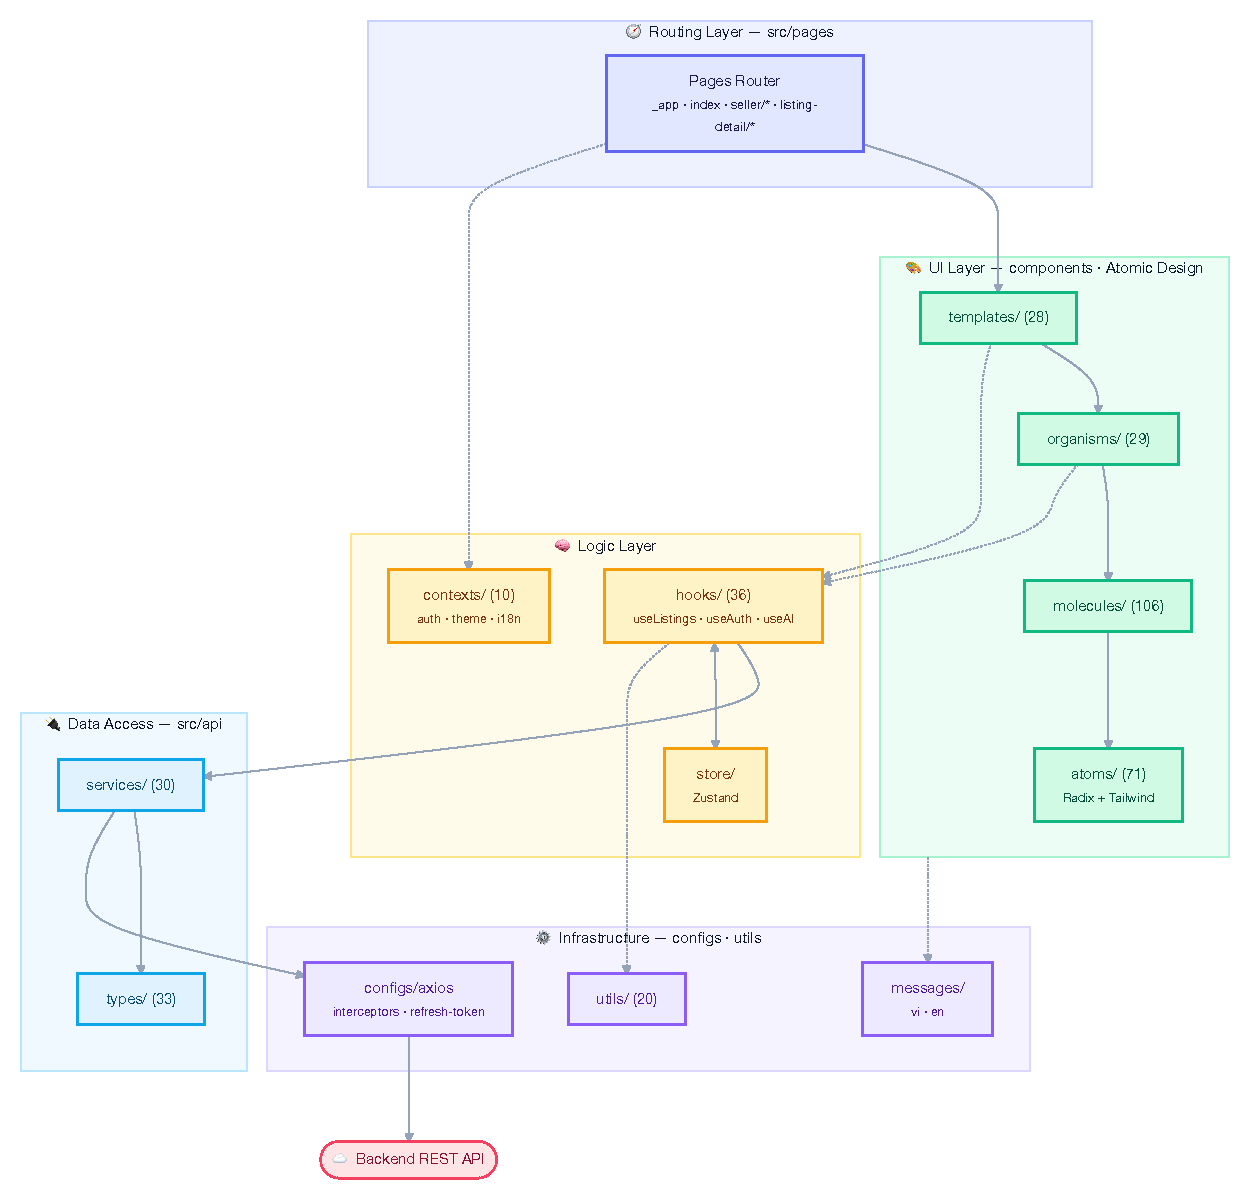
\includegraphics[width=\textwidth]{../diagrams/fe/pdf/01-architecture-layers}
\caption{Sơ đồ tổ chức mã nguồn ứng dụng web (webapp)}
\label{fig:webapp-source-org}
\end{figure}

\subsection{Cơ chế kết nối và tích hợp}

Ứng dụng web không tự chứa dữ liệu mà kết nối tới nhiều dịch vụ phía sau thông qua các kênh giao tiếp được chuẩn hóa:

\begin{itemize}
\item \textbf{Giao tiếp HTTP với Backend chính.} Mọi yêu cầu REST đi qua một thể hiện \texttt{axios} duy nhất được cấu hình tập trung tại \texttt{src/configs/axios}. Thể hiện này gắn sẵn URL gốc của Backend (biến môi trường \texttt{URL\_API\_BASE}), tiêu đề mặc định và bộ chặn (interceptor) xử lý xác thực. Toàn bộ phản hồi được chuẩn hóa về một kiểu \texttt{ApiResponse} thống nhất để các tầng phía trên xử lý nhất quán.

\item \textbf{Xác thực bằng JWT và cơ chế làm mới token.} Bộ chặn yêu cầu tự động đính kèm access token vào tiêu đề \texttt{Authorization}. Khi token sắp hết hạn hoặc máy chủ trả về lỗi 401, hệ thống tự động gọi refresh token để lấy token mới rồi phát lại yêu cầu ban đầu một cách trong suốt với người dùng. Cơ chế này còn khử trùng lặp (deduplication) để nhiều yêu cầu đồng thời chỉ kích hoạt đúng một lần làm mới, tránh tình trạng đua tranh (race condition).

\item \textbf{Cổng chặn truy cập (middleware).} Tệp \texttt{src/middleware.ts} đóng vai trò cổng kiểm soát: nó cho phép một danh sách các tuyến công khai (trang chủ, danh sách tin, chi tiết tin, tin tức, bản đồ\ldots) và chặn các tuyến cá nhân khi người dùng chưa đăng nhập. Khi đó, người dùng được chuyển hướng kèm tham số \texttt{returnUrl} để sau khi đăng nhập có thể quay lại đúng trang đang truy cập.

\item \textbf{Bộ nhớ đệm dữ liệu máy chủ.} Toàn bộ trạng thái lấy từ máy chủ được quản lý bởi TanStack Query, giúp tự động lưu đệm, làm mới nền và đồng bộ dữ liệu giữa các thành phần. Một số dữ liệu thống kê ổn định theo ngày (ví dụ thống kê tin theo tỉnh thành) còn được lưu bền vào \texttt{localStorage} để tồn tại qua các lần tải lại trang.

\item \textbf{Kết nối dịch vụ AI bằng luồng SSE.} Trợ lý hội thoại AI kết nối tới một dịch vụ AI riêng (biến môi trường \texttt{URL\_API\_AI}) và nhận câu trả lời theo thời gian thực qua kỹ thuật Server-Sent Events -- SSE (sử dụng thư viện \texttt{fetch-event-source}). Nhờ đó nội dung trả lời hiện dần theo từng đoạn, kèm theo trạng thái công cụ mà AI đang thực thi, và người dùng có thể hủy luồng đang chạy.

\item \textbf{Thông báo thời gian thực qua WebSocket.} Các thông báo (tin được duyệt, có người quan tâm\ldots) được đẩy theo thời gian thực qua giao thức STOMP trên SockJS, kết hợp với cơ chế hỏi vòng (polling) dự phòng khi mất kết nối.

\item \textbf{Tích hợp dịch vụ bên thứ ba.} Bản đồ tin đăng tích hợp Google Maps; luồng thanh toán điều hướng sang cổng thanh toán rồi nhận lại kết quả qua một trang callback công khai để cổng có thể chuyển hướng về.
\end{itemize}

Hình~\ref{fig:webapp-data-flow} minh họa luồng dữ liệu điển hình khi thực hiện một thao tác đọc/ghi: thành phần giao diện gọi hook, hook ủy thác cho TanStack Query, qua tầng dịch vụ và \texttt{axios} (kèm bộ chặn tự đính kèm và làm mới token) trước khi tới Backend. Khi ghi dữ liệu thành công, hook chủ động vô hiệu hóa bộ đệm liên quan (\texttt{invalidateQueries}) để dữ liệu hiển thị được làm mới một cách nhất quán.

\begin{figure}[H]
\centering
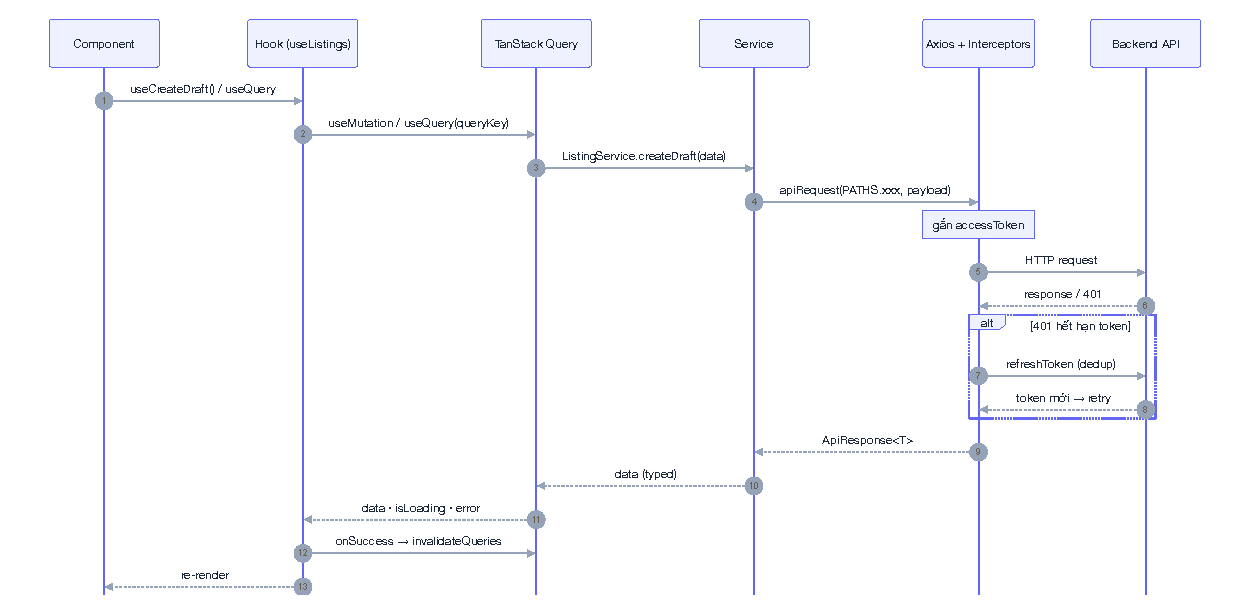
\includegraphics[width=0.92\textwidth]{../diagrams/fe/pdf/04-data-flow}
\caption{Luồng dữ liệu giữa giao diện, hook, tầng dịch vụ và Backend}
\label{fig:webapp-data-flow}
\end{figure}

\subsection{Hỗ trợ đa ngôn ngữ}

Ứng dụng hỗ trợ song ngữ tiếng Việt (mặc định) và tiếng Anh, được triển khai bằng thư viện next-intl. Mọi chuỗi hiển thị cho người dùng -- nhãn, nút bấm, thông báo, thông điệp lỗi, văn bản trạng thái rỗng -- đều không được viết cứng trong mã mà phải lấy qua các hàm \texttt{useTranslations} (phía client) hoặc \texttt{getTranslations} (phía server), tham chiếu tới hai bộ từ điển \texttt{messages/vi.json} và \texttt{messages/en.json}.

Một số điểm kỹ thuật đáng chú ý trong cơ chế đa ngôn ngữ:

\begin{itemize}
\item \textbf{Tải từ điển theo nhu cầu.} Vì phần lớn người dùng sử dụng tiếng Việt, bộ từ điển \texttt{vi.json} được đóng gói sẵn cùng ứng dụng; bộ \texttt{en.json} chỉ được tải động khi người dùng thực sự chuyển sang tiếng Anh, giúp giảm kích thước gói tải ban đầu.
\item \textbf{Bảo đảm đồng bộ khóa dịch.} Một kịch bản kiểm tra (\texttt{check-i18n-keys.js}) được chạy tự động trong bước \texttt{pre-commit} để đối chiếu sự tương đồng khóa giữa hai tệp ngôn ngữ; nếu thiếu khóa ở một ngôn ngữ, thao tác commit sẽ bị chặn.
\item \textbf{Dùng định dạng ICU.} Các chuỗi có tham số sử dụng placeholder kiểu ICU (\texttt{\{name\}}, \texttt{\{count, plural, \ldots\}}) thay vì nối chuỗi thủ công, bảo đảm đúng ngữ pháp khi trật tự từ khác nhau giữa các ngôn ngữ.
\item \textbf{Quản lý trạng thái ngôn ngữ.} Việc chuyển ngôn ngữ được điều phối qua một context riêng (\texttt{SwitchLanguageProvider}), ghi nhớ lựa chọn của người dùng và cung cấp bộ từ điển phù hợp cho toàn bộ cây thành phần.
\end{itemize}

Hình~\ref{fig:webapp-i18n} minh họa cùng một trang chủ được hiển thị ở hai ngôn ngữ: tiếng Việt (mặc định) và tiếng Anh. Người dùng có thể chuyển đổi tức thời thông qua bộ chọn ngôn ngữ trên thanh điều hướng mà không cần tải lại trang; toàn bộ nhãn, nút bấm và nội dung tĩnh đều được thay thế theo bộ từ điển tương ứng.

\begin{figure}[H]
\centering
\includegraphics[width=0.88\textwidth]{giao-dien-ngon-ngu-viet}\\[4pt]
{\small (a) Giao diện tiếng Việt}\\[10pt]
\includegraphics[width=0.88\textwidth]{giao-dien-ngon-ngu-anh}\\[4pt]
{\small (b) Giao diện tiếng Anh}
\caption{Giao diện trang chủ hiển thị ở hai ngôn ngữ tiếng Việt và tiếng Anh}
\label{fig:webapp-i18n}
\end{figure}

\subsection{Ưu điểm}

Cách tổ chức và tích hợp nêu trên mang lại một số ưu điểm rõ rệt cho nền tảng web:

\begin{itemize}
\item \textbf{Dễ bảo trì và mở rộng.} Kiến trúc Atomic Design phân lớp rõ ràng cùng việc tách logic theo nghiệp vụ giúp định vị và sửa đổi mã nhanh chóng; thêm một tính năng mới thường chỉ cần bổ sung một template, một dịch vụ và một nhóm hook tương ứng mà không ảnh hưởng phần còn lại.
\item \textbf{An toàn kiểu dữ liệu.} Việc dùng TypeScript trên toàn dự án, giới hạn kiểu \texttt{any} chỉ trong tầng định nghĩa dữ liệu truyền tải, giúp phát hiện sớm lỗi ngay khi biên dịch.
\item \textbf{Hiệu năng và trải nghiệm tốt.} Kết hợp SSR cho các trang trọng yếu về SEO, tải động (lazy loading) các thành phần nặng như bản đồ và biểu đồ, cùng cơ chế lưu đệm của TanStack Query giúp trang hiển thị nhanh và mượt.
\item \textbf{Nhất quán về giao diện.} Hệ thống thiết kế tập trung (typography, khoảng cách, màu sắc theo token ngữ nghĩa) cùng các quy tắc lint riêng bảo đảm giao diện đồng nhất giữa các trang và giữa các thành viên phát triển.
\item \textbf{Thuận lợi cho cộng tác nhóm.} Quy ước thư mục, barrel export và các cổng kiểm soát chất lượng (lint, kiểm tra kiểu, kiểm tra khóa đa ngôn ngữ) tạo nền tảng để nhiều người cùng làm việc trên cùng mã nguồn mà vẫn giữ được chất lượng ổn định.
\end{itemize}

\section{Thiết kế hệ thống Backend}

% Ghi chú: phần §3.3 do Ty + Tường phụ trách. Các sơ đồ và đoạn giải thích dưới đây
% được soạn sẵn (nháp) kèm hình minh họa; Ty + Tường rà soát, chỉnh và bổ sung nội dung.

Backend của hệ thống được xây dựng trên Spring Boot 3.4 (Java) và đóng gói thành một khối triển khai duy nhất theo mô hình Modular Monolith: toàn bộ nghiệp vụ chạy trong cùng một tiến trình nhưng được chia thành nhiều module theo miền nghiệp vụ, với ranh giới được giữ rõ ràng ở mức gói (package) và tầng dịch vụ. Cách tiếp cận này vẫn giữ được sự đơn giản khi vận hành và gỡ lỗi của một monolith, đồng thời đạt mức tách bạch đủ tốt để nhiều thành viên cùng phát triển song song.

\subsection{Kiến trúc Modular Monolith}

Hình~\ref{fig:be-architecture} mô tả kiến trúc phân lớp của Backend. Mọi yêu cầu từ web, di động hay trang quản trị đi vào qua tầng API gồm 54 controller (\texttt{@RestController}, đa số định tuyến theo tiền tố \texttt{/v1}); sau khi qua bộ lọc bảo mật, yêu cầu được chuyển xuống tầng dịch vụ (chứa toàn bộ logic nghiệp vụ), rồi tới tầng truy xuất dữ liệu (\texttt{repository}) và cơ sở dữ liệu MySQL. Bao quanh các tầng là những mối quan tâm xuyên suốt (cross-cutting): xác thực OAuth2 kết hợp JWT, bộ đệm Redis và cơ chế chịu lỗi Resilience4j.

\begin{figure}[H]
\centering
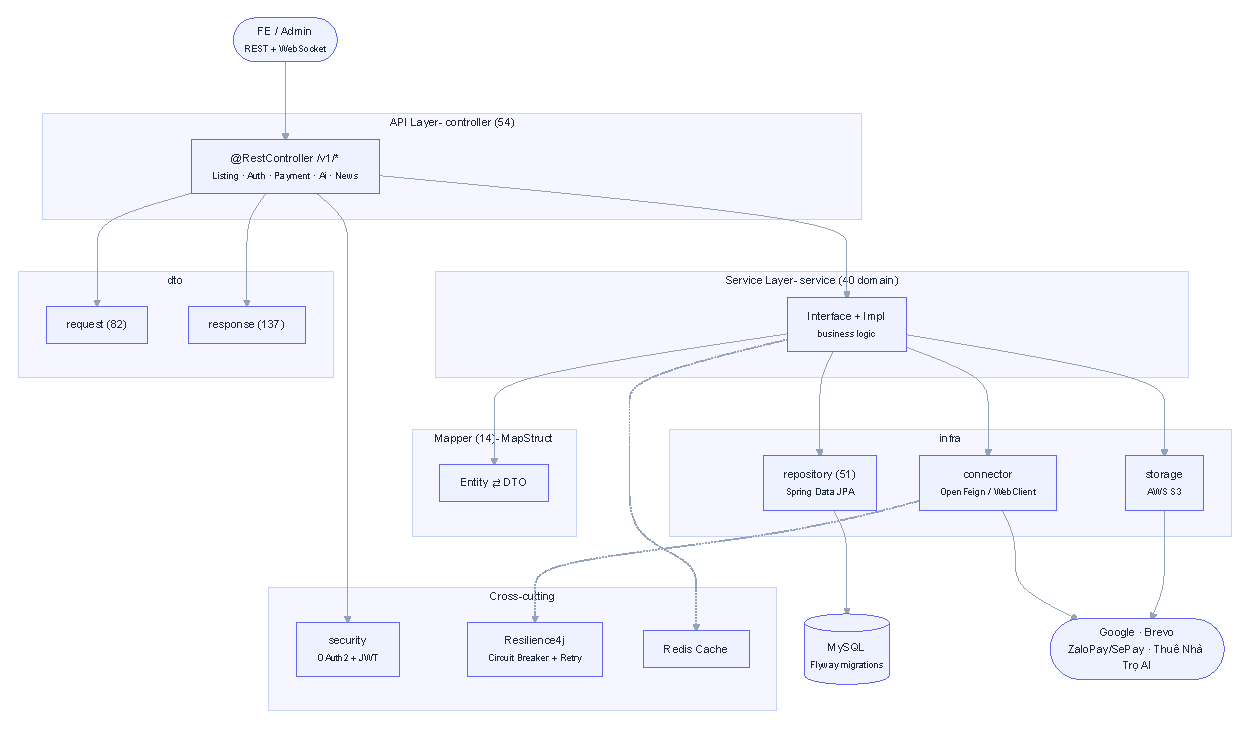
\includegraphics[width=\textwidth]{../diagrams/be/pdf/01-architecture-layers}
\caption{Kiến trúc phân lớp của hệ thống Backend (Modular Monolith)}
\label{fig:be-architecture}
\end{figure}

Tuy là một monolith nhưng hệ thống không cô lập: nó kết nối tới nhiều dịch vụ bên ngoài thông qua tầng \texttt{connector} (OpenFeign/WebClient) và \texttt{storage}, như tóm tắt ở Hình~\ref{fig:be-integrations} -- gồm MySQL, Redis, lưu trữ đối tượng (S3), đăng nhập và định vị qua Google, gửi email (Brevo), cổng thanh toán (ZaloPay/SePay) và dịch vụ AI riêng.

\begin{figure}[H]
\centering
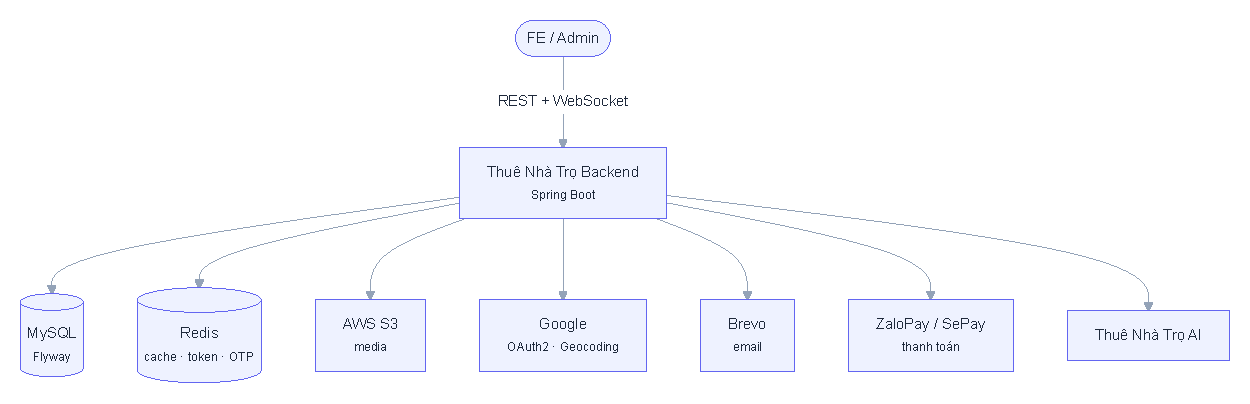
\includegraphics[width=0.95\textwidth]{../diagrams/be/pdf/05-external-integrations}
\caption{Các dịch vụ bên ngoài mà Backend tích hợp}
\label{fig:be-integrations}
\end{figure}

\subsection{Các module nghiệp vụ}

Phần nghiệp vụ được chia thành khoảng 40 module dịch vụ, mỗi module phụ trách một miền độc lập. Hình~\ref{fig:be-domains} nhóm các module theo năm cụm chức năng chính: (i) nghiệp vụ cốt lõi về tin đăng, danh mục, tìm kiếm và định giá; (ii) người dùng và xác thực; (iii) thanh toán và gói thành viên; (iv) tương tác và nội dung (thông báo, email, tin tức, AI); và (v) vận hành (quản trị, kiểm duyệt, thống kê hành vi).

\begin{figure}[H]
\centering
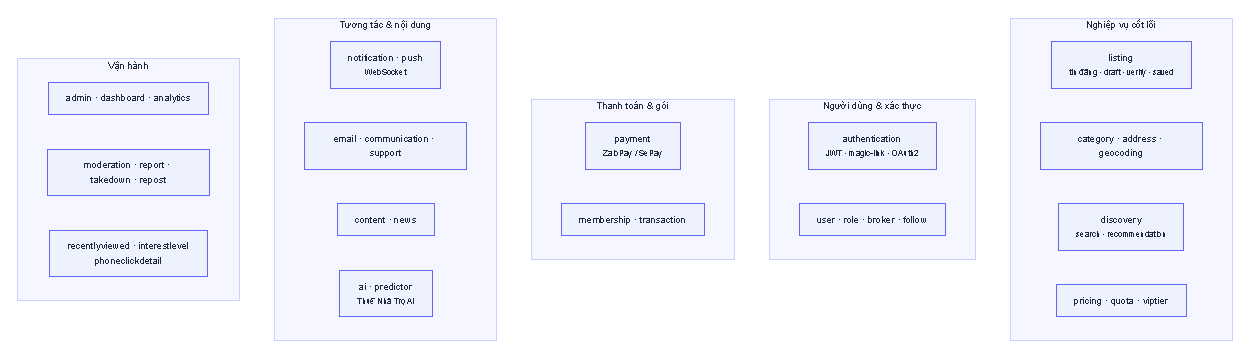
\includegraphics[width=\textwidth]{../diagrams/be/pdf/04-domain-modules}
\caption{Các module nghiệp vụ của Backend gom theo cụm chức năng}
\label{fig:be-domains}
\end{figure}

\subsection{Tổ chức phân tầng bên trong module}

Bên trong mỗi module, mã nguồn tuân theo cùng một khuôn phân tầng nhất quán, phản ánh qua cấu trúc gói \texttt{com.smartrent} ở Hình~\ref{fig:be-packages}. Tầng \texttt{controller} chỉ tiếp nhận yêu cầu và kiểm tra hợp lệ dữ liệu (\texttt{@Valid}); tầng \texttt{service} (tách giao diện và phần hiện thực \texttt{impl}) chứa logic nghiệp vụ; \texttt{mapper} (MapStruct) chuyển đổi giữa thực thể và DTO; còn \texttt{infra/repository} dùng Spring Data JPA để truy xuất dữ liệu. Các đối tượng truyền tải được tách thành \texttt{dto/request} và \texttt{dto/response}, trong khi cấu hình hệ thống (bảo mật, cache, circuit breaker, WebSocket) nằm trong gói \texttt{config}. Bảng~\ref{tab:backend-structure} liệt kê chi tiết vai trò của từng gói chính trong mã nguồn Backend.

\begin{table}[H]
\centering
\caption{Cấu trúc gói mã nguồn của Backend (\texttt{com.smartrent})}
\label{tab:backend-structure}
\begin{tabular}{|L{0.26\textwidth}|L{0.64\textwidth}|}
\hline
\textbf{Gói} & \textbf{Vai trò} \\
\hline
\texttt{controller/} & Lớp API: 54 lớp \texttt{@RestController} expose các REST endpoint (đa số theo tiền tố \texttt{/v1}); tiếp nhận yêu cầu, kiểm tra hợp lệ dữ liệu và ủy thác cho tầng dịch vụ. \\
\hline
\texttt{service/} & Lớp nghiệp vụ: 40 module theo miền (tin đăng, xác thực, thanh toán, AI\ldots), mỗi module tách \textit{giao diện} và phần \textit{hiện thực} (\texttt{impl}). \\
\hline
\texttt{dto/} & Đối tượng truyền tải, tách \texttt{request} (82) và \texttt{response} (137); cách ly mô hình API khỏi thực thể cơ sở dữ liệu. \\
\hline
\texttt{mapper/} & 14 bộ chuyển đổi (MapStruct) giữa thực thể (entity) và DTO. \\
\hline
\texttt{infra/} & Hạ tầng truy xuất dữ liệu và tích hợp: \texttt{repository} (51 -- Spring Data JPA), \texttt{connector} (gọi dịch vụ ngoài qua OpenFeign/WebClient), \texttt{storage} (S3), \texttt{client}. \\
\hline
\texttt{config/} & Cấu hình hệ thống: \texttt{security} (OAuth2 + JWT), \texttt{cache} (Redis), \texttt{circuitbreaker} (Resilience4j), WebSocket, S3 và cổng thanh toán. \\
\hline
\texttt{enums/}, \texttt{constants/} & 31 kiểu liệt kê và các hằng số nghiệp vụ dùng chung. \\
\hline
\texttt{exception/} & Các ngoại lệ nghiệp vụ và bộ xử lý lỗi tập trung (\texttt{GlobalPaymentExceptionHandler}). \\
\hline
\texttt{cronjob/} & Tác vụ định kỳ: tự kiểm duyệt tin bằng AI, thông báo tin sắp hết hạn, làm mới bộ đệm thống kê trang chủ. \\
\hline
\texttt{util/}, \texttt{utility/}, \texttt{validator/} & Hàm tiện ích (sinh \texttt{Snowflake} ID, chuẩn hóa văn bản tìm kiếm, dựng email, che dữ liệu nhạy cảm) và bộ kiểm tra ràng buộc (số tiền, hạn mức). \\
\hline
\end{tabular}
\end{table}

Cấu trúc gói nói trên được minh họa trực quan ở Hình~\ref{fig:be-packages}.

\begin{figure}[H]
\centering
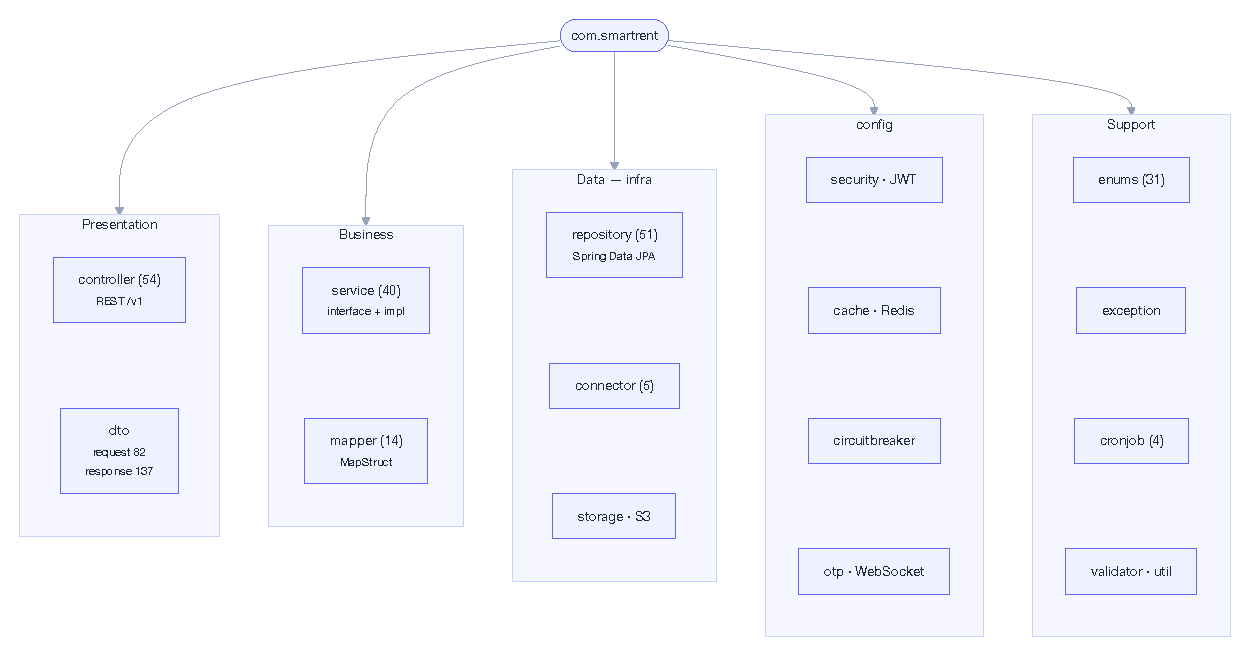
\includegraphics[width=\textwidth]{../diagrams/be/pdf/02-package-structure}
\caption{Cấu trúc gói \texttt{com.smartrent} và cách phân tầng}
\label{fig:be-packages}
\end{figure}

\subsection{Luồng dữ liệu}

Hình~\ref{fig:be-request-flow} minh họa luồng xử lý một yêu cầu có xác thực. Yêu cầu kèm \textit{Bearer token} trước hết đi qua bộ lọc bảo mật để \texttt{CustomJwtDecoder} kiểm tra token; controller kiểm tra hợp lệ DTO rồi gọi service. Service ưu tiên đọc từ bộ đệm Redis, chỉ truy vấn cơ sở dữ liệu khi \textit{cache miss} và ghi lại kết quả vào đệm; sau đó dùng mapper chuyển thực thể sang DTO phản hồi và trả về cho client dưới dạng \texttt{ApiResponse} JSON.

\begin{figure}[H]
\centering
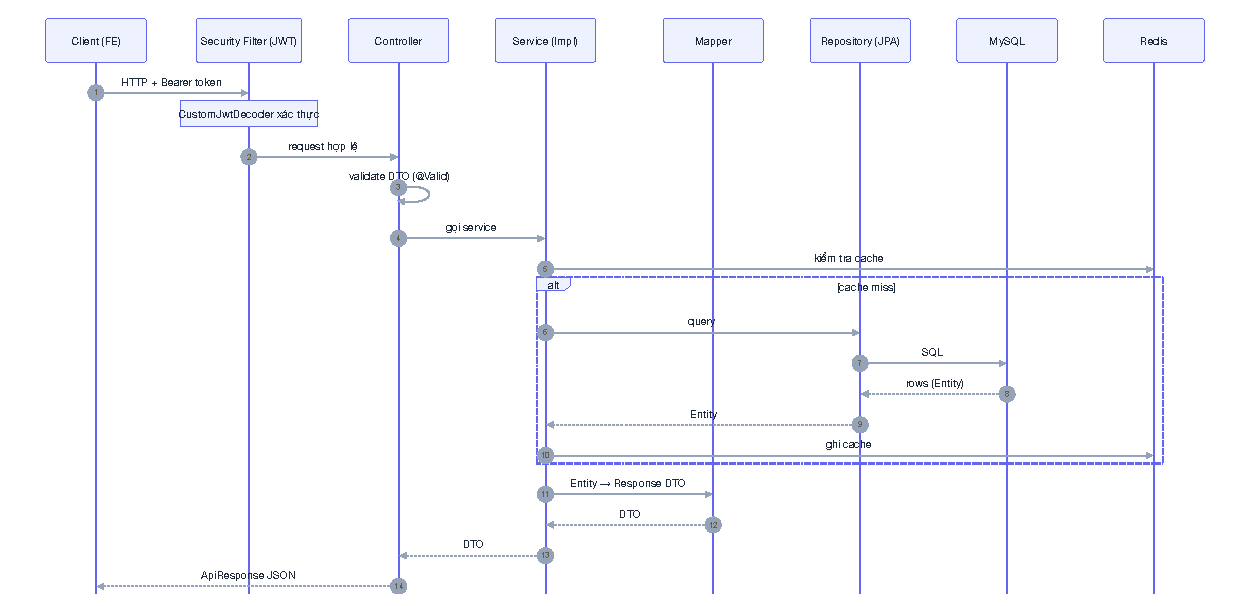
\includegraphics[width=\textwidth]{../diagrams/be/pdf/03-request-flow}
\caption{Luồng xử lý một yêu cầu có xác thực ở Backend}
\label{fig:be-request-flow}
\end{figure}

\subsection{Ưu điểm}

Mô hình Modular Monolith mang lại một số ưu điểm cho Backend của hệ thống:

\begin{itemize}
\item \textbf{Đơn giản khi vận hành.} Một khối triển khai duy nhất giúp việc build, kiểm thử và gỡ lỗi dễ dàng, đồng thời giảm chi phí hạ tầng so với kiến trúc microservices.
\item \textbf{Tách bạch theo miền.} Ranh giới module rõ ràng cho phép nhiều thành viên cùng phát triển song song mà ít giẫm chân lên nhau.
\item \textbf{Nhất quán phân tầng.} Cùng một khuôn \texttt{controller--service--repository} ở mọi module giúp mã dễ đọc, dễ bảo trì và rút ngắn thời gian làm quen cho thành viên mới.
\item \textbf{Chịu lỗi và hiệu năng.} Bộ đệm Redis giảm tải truy vấn cơ sở dữ liệu, còn Resilience4j (circuit breaker và retry) cô lập sự cố từ các dịch vụ bên ngoài, giữ hệ thống ổn định.
\item \textbf{Bảo mật tập trung.} Cơ chế xác thực OAuth2 kết hợp JWT được áp dụng thống nhất ở tầng lọc, tách khỏi logic nghiệp vụ.
\end{itemize}

\section{Thiết kế kiến trúc AI}

% TODO: Nội dung (mục mới bổ sung theo cấu trúc báo cáo).

\subsection{Luồng xử lý AI Chatbot}

% TODO: Nội dung.

\subsection{Luồng gợi ý phòng trọ}

% TODO: Nội dung.

\subsection{Tích hợp API AI}

% TODO: Nội dung.

\subsection{Kiến trúc tích hợp AI}

% TODO: Nội dung.

\section{Thiết kế cơ sở dữ liệu}

% TODO: Nội dung.

\subsection{Giới thiệu tổng quan}

% TODO: Nội dung.

\subsection{Sơ đồ thiết kế cơ sở dữ liệu của hệ thống chính}

% TODO: Nội dung.

\subsection{Mô tả chi tiết các bảng}

% TODO: Nội dung.

\section{Thiết kế giao diện}

% TODO: Nội dung (mục mới bổ sung theo cấu trúc báo cáo).

\subsection{Giao diện người thuê}

Giao diện dành cho người thuê được thiết kế đáp ứng (responsive) trên mọi kích thước màn hình, lấy người tìm trọ làm trung tâm của hành trình trải nghiệm. Toàn bộ giao diện kế thừa một hệ thống thiết kế (design system) thống nhất: bảng màu, kiểu chữ, bo góc và khoảng cách đều được khai báo dưới dạng \textit{token ngữ nghĩa} thông qua các biến CSS (CSS custom properties) trong \texttt{styles/globals.css}, thay vì gán giá trị màu cứng tại từng thành phần. Nhờ đó, hệ thống hỗ trợ sẵn hai chế độ sáng/tối (light/dark) chỉ bằng cách hoán đổi nhóm biến, và giữ được sự đồng nhất về thị giác giữa các trang cũng như giữa các thành viên phát triển.

Về kiểu chữ, ứng dụng dùng bộ phông hỗ trợ tốt cả tiếng Việt lẫn tiếng Anh (Be~Vietnam~Pro làm phông chính, Inter và Plus~Jakarta~Sans cho tiêu đề), tải qua cơ chế tối ưu phông của Next.js để tránh hiện tượng nhấp nháy khi tải. Các thành phần giao diện được xây trên nền shadcn/ui kết hợp Tailwind CSS v4, bảo đảm khả năng truy cập (accessibility) và tính nhất quán của nút bấm, biểu mẫu, hộp thoại, thẻ thông tin\ldots

Bố cục chung của khu vực người thuê được gói trong một \textit{layout} dùng lại cho hầu hết các trang, gồm: thanh điều hướng trên cùng (header) chứa logo, thanh tìm kiếm, bộ chuyển ngôn ngữ, chuông thông báo và khu vực tài khoản; phần nội dung ở giữa; chân trang (footer) với các liên kết phụ trợ; và một thanh nổi so sánh hiển thị khi người dùng đang chọn tin để đối chiếu. Cách bố trí này giúp người dùng luôn truy cập nhanh các chức năng cốt lõi ở bất kỳ trang nào.

Một số nguyên tắc thiết kế giao diện được áp dụng xuyên suốt khu vực người thuê:

\begin{itemize}
\item \textbf{Phản hồi trạng thái rõ ràng.} Mỗi thao tác bất đồng bộ đều có trạng thái tương ứng: khung chờ dạng \textit{skeleton} khi đang tải dữ liệu, chỉ báo tiến trình khi chuyển trang, thông báo lỗi thân thiện và \textit{trạng thái rỗng} có hướng dẫn khi không có kết quả.
\item \textbf{Tải động thành phần nặng.} Các khối tốn tài nguyên như bản đồ, biểu đồ lịch sử giá và danh sách tin tương tự được tải động (lazy loading) kèm khung chờ, giúp nội dung chính hiển thị nhanh mà không bị chặn.
\item \textbf{Bố cục thích ứng.} Trên màn hình lớn, trang danh sách tin dùng bố cục hai cột (bộ lọc cạnh kết quả); trên thiết bị di động, bộ lọc thu gọn vào hộp thoại trượt để tiết kiệm không gian.
\item \textbf{Đa ngôn ngữ.} Mọi nhãn, thông báo và văn bản hiển thị đều đi qua lớp đa ngôn ngữ Việt~--~Anh, cho phép chuyển đổi tức thời mà không cần tải lại trang; việc đổi ngôn ngữ chỉ thay đổi nội dung chữ, không đổi đơn vị tiền tệ của giá.
\end{itemize}

Các màn hình chính của người thuê -- trang chủ, danh sách/tìm kiếm tin, chi tiết tin đăng, bản đồ, so sánh, tin đã lưu, trang theo dõi người đăng và tin tức -- đều tuân theo cùng bộ nguyên tắc trên; kết quả hiện thực cụ thể của từng màn hình được trình bày ở Chương~\ref{Chapter5} (phần kết quả giao diện dành cho người thuê).

\subsection{Giao diện chủ trọ}

% TODO: Nội dung.

\subsection{Giao diện quản trị}

% TODO: Nội dung.

\subsection{Giao diện chatbot AI}

% TODO: Nội dung.


\chapter{Kết quả đạt được}
\label{Chapter5}

\section{Hệ thống dành cho Người thuê}

Hệ thống dành cho người thuê được hiện thực dưới dạng một ứng dụng web đáp ứng (responsive), phục vụ toàn bộ hành trình của người tìm trọ: từ khám phá, tìm kiếm, xem chi tiết, so sánh, lưu tin cho tới liên hệ trực tiếp với chủ trọ/môi giới. Phần này trình bày các kết quả chính đã đạt được trên ứng dụng web. Các tính năng AI tích hợp trong ứng dụng (trợ lý hội thoại, gợi ý cá nhân hóa\ldots) được trình bày chi tiết ở phần kết quả triển khai các tính năng AI; ở đây chỉ mô tả phần tích hợp và trải nghiệm phía giao diện.

\subsection{Trang chủ và khám phá tin đăng}

Trang chủ đóng vai trò điểm vào, tổng hợp nhiều khối nội dung giúp người dùng nhanh chóng định hướng: thanh tìm kiếm với bộ lọc nhanh theo địa điểm, loại hình và khoảng giá; khối thống kê tin đăng theo các tỉnh thành tiêu biểu (Hà Nội, Hồ Chí Minh, Đà Nẵng\ldots); khối các loại hình cho thuê phổ biến; các nhóm tin nổi bật phân theo hạng VIP; khối tin gợi ý cá nhân hóa cho người dùng đã đăng nhập; và khối tin tức mới nhất. Các số liệu thống kê được lưu đệm theo ngày để giảm tải cho máy chủ và bảo đảm trang chủ hiển thị tức thì.

\subsection{Tìm kiếm và lọc tin đăng}

Trang danh sách tin đăng cung cấp khả năng tìm kiếm và lọc đa tiêu chí, gồm: khoảng giá, diện tích, loại hình (danh mục), vị trí (tỉnh/quận/phường), số phòng ngủ -- phòng tắm, tiện ích, các loại chi phí (điện, nước, internet, phí dịch vụ), hướng nhà và sắp xếp theo nhiều tiêu chí. Toàn bộ điều kiện lọc được đồng bộ vào tham số trên thanh địa chỉ (URL), nhờ đó người dùng có thể chia sẻ hoặc lưu lại một kết quả tìm kiếm cụ thể, và trạng thái lọc được khôi phục khi mở lại đường dẫn. Kết quả được phân trang và hỗ trợ bố cục hai cột (danh sách kèm bộ lọc bên cạnh) trên màn hình lớn.

% TODO (Phát): chèn Hình -- Ảnh chụp trang tìm kiếm và bộ lọc tin đăng (ch51-search.png).

\subsection{Trang chi tiết tin đăng}

Trang chi tiết được kết xuất phía máy chủ (SSR) nhằm tối ưu SEO và tốc độ hiển thị lần đầu. Trang trình bày đầy đủ thông tin của một tin đăng: thư viện ảnh/video, tiêu đề và giá, danh sách tiện ích, mô tả chi tiết, biểu đồ lịch sử giá, bản đồ vị trí, và thẻ liên hệ chủ trọ/môi giới với chức năng hiện số điện thoại (có ghi nhận lượt bấm) cùng liên kết nhắn tin nhanh. Ở cuối trang còn có khối tin tương tự và khối tin vừa xem để gợi mở lựa chọn cho người dùng. Các thành phần nặng như bản đồ, biểu đồ và danh sách tin tương tự được tải động kèm khung chờ (skeleton) để không làm chậm phần nội dung chính.

% TODO (Phát): chèn Hình -- Ảnh chụp trang chi tiết tin đăng (ch51-detail.png).

\subsection{Bản đồ tin đăng}

Bên cạnh chế độ danh sách, người dùng có thể duyệt tin trên bản đồ (tích hợp Google Maps). Hệ thống định vị người dùng (hoặc dùng vị trí mặc định), gom nhóm các điểm tin gần nhau (marker clustering) để hiển thị gọn gàng, và đồng bộ danh sách tin trong khung nhìn hiện tại với một bảng bên cạnh. Khi người dùng di chuyển hoặc thu phóng bản đồ, hệ thống chỉ tải bổ sung tin cho vùng mới và lưu đệm các vùng đã tải để tránh gọi lại API không cần thiết, giúp thao tác trên bản đồ mượt mà.

\subsection{So sánh tin đăng}

Người dùng có thể chọn tối đa ba tin đăng để so sánh song song theo các thuộc tính quan trọng (giá, diện tích, số phòng, tiện ích, địa chỉ, các loại chi phí, hạng tin\ldots). Danh sách so sánh được lưu tạm trong phiên làm việc của trình duyệt, hiển thị dưới dạng bảng đối chiếu trực quan giúp người dùng ra quyết định nhanh hơn.

\subsection{Lưu tin và theo dõi người đăng}

Đối với người dùng đã đăng nhập, hệ thống cho phép \textit{lưu tin yêu thích} và quản lý chúng trong một trang riêng có phân trang. Ngoài ra, người dùng có thể \textit{theo dõi} các chủ trọ/môi giới và xem bảng tin tổng hợp các tin đăng từ những người mình theo dõi, với giao diện chia thành hai thẻ ``danh sách người theo dõi'' và ``bảng tin''. Đây là các tính năng tạo nên trải nghiệm cá nhân hóa và khuyến khích người dùng quay lại.

\subsection{Trợ lý hội thoại AI trên giao diện}

Ứng dụng tích hợp một widget trợ lý AI dạng nút nổi, có thể mở rộng thành cửa sổ hội thoại trên màn hình lớn hoặc toàn màn hình trên thiết bị di động. Về phía giao diện, widget nhận câu trả lời theo luồng thời gian thực (hiển thị dần từng đoạn kèm trạng thái xử lý), cho phép người dùng bấm vào các tin đăng do AI gợi ý để mở ngay hộp thoại chi tiết, ghi nhớ hội thoại trong phiên và hỗ trợ hủy luồng đang chạy. Năng lực xử lý ngôn ngữ và tìm kiếm phía sau của trợ lý được trình bày ở phần kết quả AI.

\subsection{Đăng nhập và xác thực}

Hệ thống cung cấp hai phương thức đăng nhập thuận tiện, không mật khẩu: \textit{liên kết ma thuật} (magic link) gửi qua email và \textit{đăng nhập bằng Google} (OAuth). Hộp thoại đăng nhập được thiết kế để bật lên ngay tại chỗ khi người dùng truy cập một chức năng yêu cầu xác thực, và sau khi đăng nhập thành công sẽ đưa người dùng trở lại đúng trang đang thao tác nhờ cơ chế \texttt{returnUrl}. Phiên đăng nhập được duy trì an toàn bằng cặp access/refresh token và tự động làm mới.

\subsection{Tin tức và thông báo}

Chuyên mục tin tức cung cấp danh sách bài viết có lọc theo chuyên mục, tìm kiếm theo từ khóa, bài nổi bật, khối ``xem nhiều nhất'' và trang chi tiết bài viết (kết xuất SSR). Bên cạnh đó, người dùng đã đăng nhập nhận được \textit{thông báo thời gian thực} qua WebSocket (kèm hỏi vòng dự phòng) về các sự kiện liên quan như tin được duyệt hay có tương tác, cùng chỉ báo số thông báo chưa đọc.

\subsection{Trải nghiệm đa thiết bị và đa ngôn ngữ}

Toàn bộ các trang trên đều được thiết kế đáp ứng cho cả máy tính và thiết bị di động, hỗ trợ song ngữ Việt -- Anh và chuyển đổi tức thời. Các yếu tố như chỉ báo tiến trình tải trang, khung chờ khi tải dữ liệu, trạng thái rỗng có hướng dẫn rõ ràng và chuyển đổi đơn vị tiền tệ theo ngôn ngữ góp phần tạo nên trải nghiệm liền mạch và chuyên nghiệp cho người thuê.

% TODO (Phát): chèn Hình -- Ảnh chụp giao diện webapp trên máy tính và di động (ch51-responsive.png).

\section{Hệ thống dành cho Quản trị viên}

% TODO: Nội dung.

\subsection{Thống kê \& Giám sát Hệ thống}

% TODO: Nội dung.

\subsection{Quản lý Người dùng \& Phân quyền}

% TODO: Nội dung.

\subsection{Quản lý tin đăng và kiểm duyệt nội dung}

% TODO: Nội dung.

\subsection{Quản lý doanh thu và thanh toán}

% TODO: Nội dung.

\section{Kết quả triển khai các tính năng AI}

% TODO: Nội dung.

\subsection{AI Agent hỗ trợ tìm kiếm nhà trọ}

% TODO: Nội dung.

\subsection{AI đánh giá giá bất động sản}

% TODO: Nội dung.

\subsection{AI tạo nội dung bài đăng}

% TODO: Nội dung.

\subsection{Hệ thống gợi ý cá nhân hóa}

% TODO: Nội dung.

\subsection{AI kiểm duyệt nội dung bài đăng}

% TODO: Nội dung.


\chapter{Kết luận và hướng phát triển}
\label{Chapter7}

\section{Kết quả đạt được}

% TODO: Nội dung (phần này còn để trống trong file Báo Cáo Cuối Kỳ).

\section{Kiến thức và kinh nghiệm thu nhận được}

% TODO: Nội dung.

\subsection{Về mặt kỹ thuật}

% TODO: Nội dung.

\subsection{Về kỹ năng làm việc nhóm và lập kế hoạch}

% TODO: Nội dung.

\subsection{Một số kiến thức và kinh nghiệm khác}

% TODO: Nội dung.

\section{Hạn chế của hệ thống}

% TODO: Nội dung.

\section{Hướng phát triển}

% TODO: Nội dung.


% Công trình của tác giả (nếu không có thì comment 02 dòng dưới)
% \addcontentsline{toc}{chapter}{Danh mục công trình của tác giả}
% \include{Appendix/publish}

% In tài liệu tham khảo
\addcontentsline{toc}{chapter}{Tài liệu tham khảo}
\printbibheading[title={Tài liệu tham khảo}]



%\printbibliography

\printbibliography[heading=subbibliography, title={Tiếng Việt}, keyword=Viet, resetnumbers=true]

\DeclareNameAlias{sortname}{last-first}
\DeclareNameAlias{default}{last-first}

\printbibliography[heading=subbibliography, title={Tiếng Anh}, notkeyword=Viet, resetnumbers=7]
% ===================================================================== %
% CHÚ Ý: phải gán lại resetnumbers=số tài liệu tham khảo tiếng Việt + 1 %
% ===================================================================== %

\end{document}
